%% ===========================================================================
%%  Gradient at the Edge of Chaos
%%  Journal of Automation and Intelligence submission build.
%%  Elsevier CAS bundle, double-column class (cas-dc). To switch to the
%%  single-column layout, change the \documentclass line below to
%%  cas-sc -- the section files under sections/ are class-independent.
%% ===========================================================================
\documentclass[a4paper,fleqn]{cas-dc}

% ---- bibliography: numbered (Vancouver-style) references -----------------
\usepackage[numbers,sort&compress]{natbib}

% ---- math ---------------------------------------------------------------------
\usepackage{bm}
\usepackage{mathtools}

% ---- units ------------------------------------------------------------------
\usepackage{siunitx}
\sisetup{detect-weight=true,detect-family=true}

% ---- algorithms -------------------------------------------------------------
\usepackage[ruled,vlined,linesnumbered]{algorithm2e}
\providecommand{\textproc}[1]{\textsc{#1}}

% ---- diagrams -------------------------------------------------------------
\usepackage{tikz}
\usetikzlibrary{arrows.meta,positioning,fit,backgrounds,calc,shapes.geometric,shapes.misc}

\tikzset{
  block/.style   = {draw, rounded corners=2pt, align=center, font=\small,
                     minimum height=8mm, inner sep=4pt, fill=blue!4},
  envblock/.style = {draw, rounded corners=2pt, align=center, font=\small,
                     minimum height=8mm, inner sep=4pt, fill=green!6},
  anblock/.style  = {draw, rounded corners=2pt, align=center, font=\small,
                     minimum height=8mm, inner sep=4pt, fill=red!6},
  databox/.style  = {draw, align=center, font=\small, minimum height=8mm,
                     inner sep=4pt, fill=gray!8},
  flow/.style     = {-{Latex[length=2mm]}, thick},
  grad/.style     = {-{Latex[length=2mm]}, thick, dashed, red!70!black},
}

% ---- misc -----------------------------------------------------------------
\usepackage{microtype}
\emergencystretch=2em
\usepackage{cleveref}
\crefname{equation}{Eq.}{Eqs.}
\crefname{figure}{Fig.}{Figs.}
\crefname{table}{Table}{Tables}
\crefname{section}{Section}{Sections}
\crefname{algocf}{Algorithm}{Algorithms}

% ---- CAS class tweaks ---------------------------------------------------------
% (a) name the target journal in the first-page footer (default: "Elsevier")
% (b) print the "ORCID(s):" footnote line only when an ORCID is actually given
\ExplSyntaxOn
\cs_set:Npn \__first_footerline:
  {
    \group_begin:
      \small \sffamily
      \ifnum\theblind>0\relax\else \__short_authors: :~ \fi
      { \rmfamily \itshape Journal~of~Automation~and~Intelligence }
    \group_end:
  }
\cs_set:Npn \printorcid
  {
    \seq_if_empty:NF \g_stm_orcid_seq
      {
        \group_begin:
          \tex_let:D \thefootnote \relax \footnotetext
            {
              \raggedright
              \textsc{orcid}(s):\c_space_token
              \seq_use:Nn \g_stm_orcid_seq { ;~ }
            }
        \group_end:
      }
  }
\ExplSyntaxOff

% ---- notation shorthands (used across sections/) --------------------------
\renewcommand{\Re}{\mathit{Re}}
\newcommand{\gan}{g_{\mathrm{an}}}
\newcommand{\Lan}{\mathcal{L}_{\mathrm{an}}}
\newcommand{\dd}{\mathrm{d}}

\graphicspath{{figures/}}

\begin{document}
\let\WriteBookmarks\relax
\def\floatpagepagefraction{1}
\def\textpagefraction{.001}

\shorttitle{Gradient at the edge of chaos}
\shortauthors{C. \"Ozkurt et~al.}

\title[mode = title]{Gradient at the Edge of Chaos: Why Analytic-Gradient
Reinforcement Learning Has No Seed-Robust Advantage on Chaotic Kolmogorov Flow}

\author[1]{Cem \"Ozkurt}[orcid=0000-0002-1251-7715]
\cormark[1]
\ead{cemozkurt@sakarya.edu.tr}
\credit{Conceptualization, Methodology, Investigation,
Writing -- original draft, Project administration}

\author[2]{Muhammed Emin Onay}[orcid=0009-0000-0454-4986]
\credit{Data curation, Visualization, Investigation,
Writing -- review \& editing}

\author[2]{Ey\"up Altu\u{g} Tun\c{c}}[orcid=0009-0007-5166-8077]
\credit{Software, Validation, Investigation,
Writing -- review \& editing}

\author[3]{Ahmet Kutay K\"u\c{c}\"ukler}[orcid=0009-0007-0202-016X]
\credit{Investigation, Validation, Writing -- review \& editing}

\author[3]{Haktan Yusuf G\"ulo\u{g}lu}[orcid=0009-0007-9429-6154]
\credit{Conceptualization, Software, Formal analysis, Resources,
Writing -- original draft, Writing -- review \& editing}

\affiliation[1]{organization={Department of Data Science and Analytics,
Faculty of Computer and Information Sciences, Sakarya University},
                addressline={Esentepe Campus, Serdivan},
                postcode={54187},
                city={Sakarya},
                country={T\"urkiye}}

\affiliation[2]{organization={Department of Computer Engineering,
Faculty of Computer and Information Sciences, Sakarya University},
                addressline={Esentepe Campus, Serdivan},
                postcode={54187},
                city={Sakarya},
                country={T\"urkiye}}

\affiliation[3]{organization={Department of Computer Engineering,
Sakarya University of Applied Sciences},
                city={Sakarya},
                country={T\"urkiye}}

\cortext[1]{Corresponding author.}

\begin{abstract}
Does injecting an analytic
(backpropagated-through-the-simulator) policy gradient help or hurt as a
fluid-flow control task becomes chaotic, and does off-policy reinforcement
learning (RL) tolerate the resulting gradient instability better than
on-policy RL? The HydroGym paper reports that Gradient-Enhanced PPO (GPPO)
cuts training iterations by at least \SI{65}{\percent} relative to PPO, shown
at a single Reynolds number and seed. We evaluate PPO, GPPO, SAC, and a
gradient-enhanced SAC variant (GSAC), the first transfer of off-policy
maximum-entropy analytic-gradient RL to fluid dynamics, on the real
\mbox{\texttt{hydrogym.jax}} Kolmogorov-flow environment at a regular
($\Re=45$) and a chaotic ($\Re=300$) operating point over five seeds. At
$\Re=45$, GPPO reaches PPO's best reward in substantially fewer episodes in 4
of 5 seeds, reproducing the reported mechanism. At $\Re=300$, all four
algorithms eventually diverge, and the first-divergence episode is dominated
by the seed, not the algorithm: an exact permutation test separates no pair
of algorithms (all $p\ge 0.19$). The reproducible findings are mechanistic:
the break is sudden and precursor-free; the replay buffer's size at the
trigger determines whether a brief post-trigger survival window can appear;
and in a rare mode the flow diverges within about two episodes regardless of
algorithm. Analytic-gradient injection thus imposes no seed-robust ordering
on chaotic-regime training stability.
\end{abstract}

\begin{highlights}
\item GSAC is the first off-policy analytic-gradient RL applied to Kolmogorov flow.
\item At $\Re=45$, GPPO reproduces the reported sample-efficiency gain (63--84\%).
\item At $\Re=300$ all four algorithms diverge; the breaking episode is seed-dominated.
\item An exact permutation test separates no pair of algorithms (all $p\ge0.19$).
\item The chaotic-regime break is sudden, precursor-free and replay-buffer gated.
\end{highlights}

% JAI Guide for Authors: maximum of 6 keywords.
\begin{keywords}
analytic policy gradients \sep differentiable simulation \sep
reinforcement learning for flow control \sep chaotic dynamics \sep
training stability \sep Kolmogorov flow
\end{keywords}

\maketitle

\section{Introduction}
\label{sec:intro}

The active control of fluid flows --- for drag reduction, mixing
enhancement, or extreme-event suppression --- is one of the areas where
machine learning has changed computational fluid
dynamics~\cite{brunton2020mlfluid,vinuesa2022enhancing} most directly, and
reinforcement learning (RL) is now one of its most active application
routes. Rabault et al.~\cite{rabault2019} first showed that deep RL can control periodic vortex
shedding behind a cylinder, achieving $\sim$\SI{8}{\percent} drag reduction
at $\Re=100$; the line has since extended into the turbulent regime, e.g.\
turbulent separation-bubble control~\cite{font2025} and real-time
state-dependent turbulent-wake control~\cite{react2026}.
HydroGym~\cite{hydrogym2026} consolidates these scattered codebases into a
single solver-agnostic platform spanning \num{61}+ environments from laminar
to turbulent and --- alongside classical solvers --- ships a JAX-based, end-to-end
\emph{differentiable} pseudo-spectral solver that continues the line of
differentiable-CFD libraries JAX-CFD~\cite{jaxcfd2021} and
JAX-Fluids~\cite{jaxfluids2022,jaxfluids2024}. A methodologically related,
PyTorch-based differentiable flow-control benchmark, FluidGym~\cite{fluidgym2026},
belongs to the same ecosystem.

Differentiability lets RL move beyond model-free training by computing
\emph{analytic policy gradients}: the derivative of the reward with respect
to the policy parameters, obtained by the chain rule \emph{through the
simulator itself} rather than by sampling. The HydroGym paper demonstrates
this with GPPO, in which the analytic gradient is mixed with PPO's
likelihood-ratio gradient --- a construction closely related to
Gradient-Informed PPO~\cite{gippo2023} --- and on the Kolmogorov-flow
environment this is reported to cut training iterations by at least
\SI{65}{\percent} and to yield controllers with lower action
amplitude~\cite{hydrogym2026}. That result, however, is shown at a
\emph{single operating point} of the wide $\Re=40$--$500$ range the paper
defines for Kolmogorov flow; the behaviour of the analytic gradient at the
regular and chaotic ends of that range is not separately compared.

This gap overlaps a documented risk. Metz et al.~\cite{metz2021} demonstrate
a common ``chaos-induced failure mode'' of backpropagation through iterated
maps, physics simulations, and learned optimizers, and tie it to the
spectrum of the system Jacobian. On the fluid-dynamics side, Boffetta and
Musacchio~\cite{boffetta2017} show that the largest Lyapunov exponent of
homogeneous-isotropic turbulence grows with Reynolds number, so the
predictability horizon shrinks as $\Re$ rises. Together these two
independent results suggest that in a chaotic regime the norm and direction
of the analytic gradient can become hypersensitive to initial conditions,
and that GPPO's reported advantage could weaken, or reverse, as $\Re$
increases.

Analytic-gradient injection has so far been applied mostly with
\emph{on-policy} methods or in rigid-body robotics tasks: SHAC~\cite{shac2022}
mitigates the exploding/vanishing gradient problem with short-horizon
rollouts and a learned terminal value; AHAC~\cite{ahac2024} adapts the
horizon to avoid stiff dynamics. On the off-policy side, SAPO~\cite{sapo2025}
carries analytic-gradient RL into a maximum-entropy (SAC-like) framework and
reports strong performance on deformable-body tasks --- but this approach has
never been applied to fluid dynamics. We add GSAC, a
gradient-enhanced version of SAC~\cite{sac2018}, as a fourth method, placing
the comparison at the intersection of the SHAC family (short-horizon analytic
gradient) and the SAPO family (off-policy maximum-entropy analytic gradient),
and asking whether the off-policy replay-buffer structure tolerates
chaotic-regime gradient instability better than on-policy GPPO.

The paper makes the following contributions:
\begin{enumerate}
  \item We extend HydroGym's GPPO-vs-PPO result on Kolmogorov
  flow~\cite{hydrogym2026} from a single Reynolds point to a
  regular-vs-chaotic regime comparison, and from $n=1$ to $n=5$ seeds
  (\cref{sec:results}).
  \item We introduce GSAC (SAC $+$ short-horizon analytic
  gradient), never previously applied to HydroGym and the first transfer of
  the SAPO~\cite{sapo2025} family to fluid dynamics, giving a $2\times 2$
  design (on-/off-policy $\times$ with/without analytic gradient) that
  isolates each factor (\cref{sec:methods}).
  \item \emph{A seed-dominance result, replicated over five seeds with a
  formal test.} In the chaotic regime all four algorithms eventually
  diverge, and the episode at which they first diverge is dominated by the
  training seed, not the algorithm: each algorithm's first-NaN episode spans
  more than an order of magnitude, PPO is both the first to break at
  $\text{seed}=0$ and the most robust of the four at $\text{seed}=2$, and an
  exact sign-flip permutation test separates no pair of algorithms (all
  $p\ge 0.19$; Kruskal--Wallis $p=0.57$, Friedman $p=0.77$).
  Analytic-gradient injection does not delay the on-policy break
  (GPPO$-$PPO mean $-2.4$ episodes, $p=0.81$).
  \item \emph{Two mechanistic results that do survive}, both
  algorithm-design-independent: (a) a replay-buffer dilution calculation for
  whether a brief post-trigger ``survival window'' can appear (non-zero
  probability only for large-buffer GSAC; one window seen in \num{20} runs,
  that case); and (b) an early-init failure mode --- when the initial policy
  already sits near the solver's stability boundary the flow diverges within
  $\sim$2 episodes regardless of algorithm --- documented directly with
  per-episode action-amplitude and analytic-gradient-norm logs
  (\cref{sec:mechanism}).
  \item GSAC is characterized as highest ceiling, no reliable
  floor: 2--10$\times$ the stable horizon of any other method when training
  gets a foothold, but episode-2 failure when the flow diverges before
  learning begins.
\end{enumerate}

We pre-registered the hypothesis that the norm/variance of the analytic
gradient would be stable at low $\Re$ and unstable at high $\Re$; against
this instability, GSAC's off-policy structure would be more robust than
GPPO's on-policy structure. At $n=5$ this was not supported at $p<0.05$:
GSAC has the highest median breaking point and is most robust in 3 of 5
seeds, and GSAC$-$GPPO is positive in the mean ($+39$ episodes), but the
sign-flip permutation $p$-value is \num{0.19} and the effect is dominated by
seed-to-seed variance. Per the pre-registered decision rule (\cref{sec:sig})
the finding stands as ``no seed-robust ordering''; GSAC's lean is reported
as a candidate effect for a larger-$n$ study.

The remainder of the paper is organized as follows. \Cref{sec:related}
reviews analytic-gradient RL and chaotic-system instability.
\Cref{sec:methods} formulates the environment, the four algorithms, and the
analytic-gradient mechanism with its computation graph and algorithm boxes.
\Cref{sec:setup} gives the configuration, seed protocol, and reproducibility
package. \Cref{sec:results} reports the regular- and chaotic-regime results
and the significance test; \cref{sec:mechanism} dissects the break;
\cref{sec:discussion,sec:conclusion} discuss and conclude.

\section{Related work}
\label{sec:related}

\Cref{tab:related} positions this study against the closest prior work along
three axes: the base RL family, whether an analytic (through-simulator)
gradient is used, and whether the chaotic/turbulent regime is addressed.

\begin{table*}[tbp]
\centering
\caption{Positioning against the closest prior work. AG $=$ analytic
(through-simulator) policy gradient; ME $=$ maximum-entropy (SAC-style)
objective; \checkmark\ = present, dash = absent.}
\label{tab:related}
\footnotesize
\setlength{\tabcolsep}{4pt}
\resizebox{\textwidth}{!}{%
\begin{tabular}{|l|l|l|c|c|l|}
\hline
Work & Base & AG & ME & Chaotic & Domain \\
\hline
HydroGym / GPPO~\cite{hydrogym2026} & PPO & \checkmark & -- & one $\Re$ & Kolmogorov flow \\
\hline
GI-PPO~\cite{gippo2023}             & PPO & \checkmark (adapt.) & -- & -- & rigid body \\
\hline
RPO~\cite{rpo2025}                  & PPO & \checkmark & -- & -- & control suites \\
\hline
SHAC~\cite{shac2022}                & AC  & \checkmark (short-$H$) & -- & -- & locomotion \\
\hline
AHAC~\cite{ahac2024}                & AC  & \checkmark (adapt.-$H$) & -- & -- & contact-rich \\
\hline
SAPO~\cite{sapo2025}                & SAC & \checkmark & \checkmark & -- & rigid/deformable \\
\hline
Bucci et al.~\cite{bucci2019}       & DDPG & -- & -- & \checkmark & Kuramoto--Sivashinsky \\
\hline
Font et al.~\cite{font2025}         & PPO & -- & -- & \checkmark & separation bubble \\
\hline
This work                  & PPO, SAC & \checkmark & \checkmark & 45 / 300 & Kolmogorov flow \\
\hline
\end{tabular}%
}

\end{table*}

\subsection{RL for flow control and HydroGym}
Since Rabault et al.~\cite{rabault2019}, model-free RL has repeatedly
succeeded on turbulent flow control: separation-bubble
control~\cite{font2025} reports $\sim$\SI{9}{\percent} vs $\sim$\SI{6.8}{\percent}
reduction over classical periodic forcing; an early study~\cite{turbdrl2020}
establishes DRL's applicability to turbulent conditions; real-time
state-dependent bluff-body wake control~\cite{react2026} achieves 2--4$\times$
the performance of model-based baselines in wind-tunnel experiments; deep RL
has also learned energy-efficient collective swimming gaits by exploiting
shed vortices~\cite{verma2018vortices}. A broad
robotics survey~\cite{drlrobotics2025} documents the wider maturity of RL
for real-world control. HydroGym~\cite{hydrogym2026} unifies these under one
solver-agnostic interface, shows zero-shot policy transfer across
environments, and reports the $\ge$\SI{65}{\percent} sample-efficiency gain
for GPPO over PPO on Kolmogorov flow that this paper examines.
FluidGym~\cite{fluidgym2026} is a related PyTorch-based differentiable
benchmark with PPO/SAC baselines. None of these works systematically
compares analytic-gradient injection across a regular and a chaotic regime.

\subsection{Analytic policy gradients through differentiable simulation}
The single closest prior method to GPPO is GI-PPO~\cite{gippo2023}:
it introduces an ``$\alpha$-policy'' that adaptively weights the analytic
gradient against the PPO gradient, down-weighting the analytic term when it
is detected to be high-variance or biased. Our fixed 50/50 mix is the
non-adaptive special case ($\alpha$ held constant). RPO~\cite{rpo2025}
analyzes the on-policy analytic-gradient setting directly, showing that
reparameterization policy gradients with sample reuse optimize a PPO-style
surrogate via backpropagation-through-time (BPTT) and targeting exactly the
training instability this paper measures at $\Re=300$.
The broader family originated in robotics/control. SHAC~\cite{shac2022}
decouples the analytic gradient from the full episode horizon using
short-horizon rollouts and a smooth critic; our 6-step horizon is a direct
adaptation. AHAC~\cite{ahac2024} replaces the fixed horizon with
one adaptively truncated to avoid stiff dynamics. SAPO~\cite{sapo2025}
carries the idea into a maximum-entropy, off-policy framework, testing
whether entropy regularization smooths the analytic-gradient landscape; our
GSAC is the first application of the SAPO idea to fluid dynamics.

\subsection{Analytic-gradient instability in chaotic systems}
The theoretical basis of our hypothesis is Metz et al.~\cite{metz2021}: in
chaotic dynamical systems, backpropagated gradients explode through a
butterfly-effect mechanism rooted in the system Jacobian spectrum, with
clipping, truncated BPTT, or a switch to zeroth-order methods proposed as
remedies. Parmas et al.~\cite{parmas2018pipps} show the same failure
directly in model-based policy search: gradients through long chains of
nonlinear computation become large and effectively random in direction, and
reparameterization (analytic) gradients suffer from it while
likelihood-ratio (model-free) gradients are comparatively robust --- the
same asymmetry this paper's on-policy result partially echoes
(\cref{sec:results}). The fluid-dynamics counterpart is Boffetta and
Musacchio~\cite{boffetta2017}: the largest Lyapunov exponent (estimated in
practice via the classical time-series method of Wolf et
al.~\cite{wolf1985lyapunov}) of homogeneous-isotropic turbulence grows with
$\Re$ and the predictability horizon shrinks inversely with it. Together
these frame our 500-episode
finding that GPPO and GSAC also eventually reach NaN, only later: instability
is inevitable; what differs is only the delay mechanism. That gradient-free
RL \emph{can} control spatiotemporal chaos is not in question --- Bucci et
al.~\cite{bucci2019} do exactly this on the Kuramoto--Sivashinsky equation
--- the question here is whether \emph{analytic-gradient} injection survives
the chaotic regime.

\subsection{Analytic vs.\ zeroth-order gradients; partial differentiability}
Suh et al.~\cite{suh2022} compare analytic and zeroth-order policy gradients
in systems with stiffness and discontinuities, and via a bias--variance
analysis propose an $\alpha$-graded interpolating estimator, of which our
50/50 mix is roughly the $\alpha=0.5$ special case. A 2026
follow-up~\cite{onoda2026} re-tests the same question with a lighter
hybrid-switching scheme. ABPT~\cite{abpt2025} proposes an amended BPTT scheme
combining 0-step and $N$-step returns for partially differentiable rewards,
a problem class close to HydroGym's mixed control-reward / physics-state
structure.

\subsection{Base algorithms and distributed PDE control}
The gradient-free anchors are PPO~\cite{ppo2017} and Soft
Actor-Critic~\cite{sac2018,sacapps2018}. PPO builds on TRPO~\cite{trpo2015}
and Generalized Advantage Estimation (GAE)~\cite{gae2015}; Soft
Q-learning~\cite{softq2017} is the origin of SAC's maximum-entropy
framework; both algorithms' updates in this study use
Adam~\cite{kingma2015adam}. On the distributed structure of PDE actuation, Peitz et
al.~\cite{peitz2024} exploit translational equivariance to turn a
high-dimensional control problem into a multi-agent problem with identical
uncoupled agents; Kolmogorov flow's low-wavenumber sinusoidal actuators sit
in the same distributed-control setting.

\section{Methods}
\label{sec:methods}

\subsection{Approach}
\label{sec:approach}

Model-free reinforcement learning treats the simulator as a black box and
estimates the policy gradient from sampled returns alone. This is robust and
makes almost no assumptions, but the estimate is high-variance and
sample-hungry, and on flow-control problems it can take tens of thousands of
environment interactions to converge. When the simulator is itself
differentiable, a second route becomes available: differentiate the
accumulated reward \emph{through} the solver and obtain the policy gradient
from the chain rule directly. This \emph{analytic} (or first-order) gradient
is far lower in variance and, on smooth control problems, converges in a
fraction of the interactions. It is the mechanism behind
differentiable-physics methods such as SHAC~\cite{shac2022},
AHAC~\cite{ahac2024} and SAPO~\cite{sapo2025} in robotics, behind
differentiable-CFD control with JAX-CFD~\cite{jaxcfd2021} and
JAX-Fluids~\cite{jaxfluids2022}, and behind the GPPO result on Kolmogorov
flow that this paper follows up~\cite{hydrogym2026}.

The derivative that makes this route fast also makes it fragile.
Backpropagating through a long or stiff rollout produces gradients that
explode or vanish, and the estimate is biased whenever the horizon is
truncated or the dynamics are contact-rich or
chaotic~\cite{metz2021,suh2022}. The established mitigations are to use a
\emph{short} differentiation horizon, to forward-propagate only the
deterministic mean action so the differentiated chain stays smooth, and to
\emph{mix} the analytic gradient with the ordinary model-free gradient rather
than trust it alone~\cite{shac2022,suh2022,gippo2023}. Chaotic flow is
exactly where this fragility is expected to matter most: neighbouring
trajectories separate exponentially, so the through-solver gradient of a
many-step rollout can be swamped by noise, and the predictability horizon
shrinks as the Reynolds number rises~\cite{metz2021,boffetta2017}. Whether
the analytic gradient still helps in that regime --- and whether an
off-policy replay buffer absorbs the instability better than an on-policy
update --- is the question this study is built to answer.

The rest of this section constructs the four algorithms used to test it. We
fix a single environment and control problem (\cref{sec:env}) and cast it as
a Markov decision process (\cref{sec:mdp}); we state the two model-free
estimators, PPO and SAC (\cref{sec:ppo,sec:sac}); we then define the analytic
gradient and the fixed 50/50 mixing rule (\cref{sec:analytic}); and finally
we assemble the on-policy variant GPPO (\cref{sec:gppo}) and the off-policy
variant GSAC (\cref{sec:gsac}). The factorial design that crosses these
choices is described first.

\subsection{Overall design}
\label{sec:design}

We compare four algorithms in a $2\times 2$ factorial design that crosses the
RL family (on-policy vs.\ off-policy) with analytic-gradient injection
(absent vs.\ present), so that each factor and their interaction can be read
off directly (\cref{fig:design}). All four share one environment, one network
architecture, one optimizer, and one training budget (\cref{sec:setup}); they
are evaluated at a regular ($\Re=45$) and a chaotic ($\Re=300$) operating
point of the same Kolmogorov-flow solver.

\begin{figure*}[t]
\centering
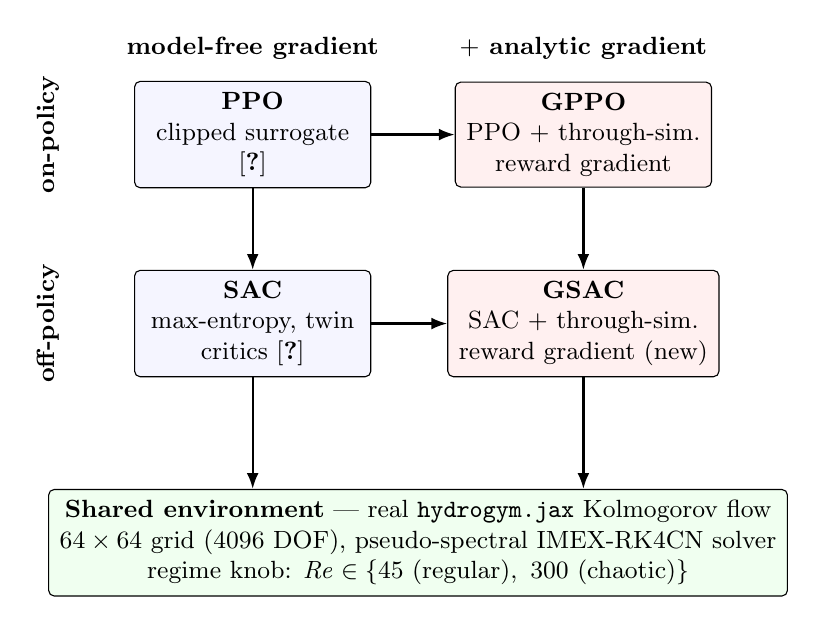
\begin{tikzpicture}[node distance=6mm]
  \node[font=\small\bfseries] (c1) at (0,2.1) {model-free gradient};
  \node[font=\small\bfseries] (c2) at (4.2,2.1) {$+$ analytic gradient};
  \node[font=\small\bfseries,rotate=90] at (-2.6,1.0) {on-policy};
  \node[font=\small\bfseries,rotate=90] at (-2.6,-1.4) {off-policy};

  \node[block,minimum width=30mm] (ppo)  at (0,1.0)  {\textbf{PPO}\\clipped surrogate\\ \cite{ppo2017}};
  \node[anblock,minimum width=30mm] (gppo) at (4.2,1.0) {\textbf{GPPO}\\PPO $+$ through-sim.\\reward gradient};
  \node[block,minimum width=30mm] (sac)  at (0,-1.4) {\textbf{SAC}\\max-entropy, twin\\critics \cite{sac2018}};
  \node[anblock,minimum width=30mm] (gsac) at (4.2,-1.4) {\textbf{GSAC}\\SAC $+$ through-sim.\\reward gradient (new)};

  \draw[flow] (ppo) -- (gppo);
  \draw[flow] (sac) -- (gsac);
  \draw[flow] (ppo) -- (sac);
  \draw[flow] (gppo) -- (gsac);

  % shared environment, centred under both columns; straight vertical edges
  \node[envblock,minimum width=76mm,anchor=north] (env) at (2.1,-3.5)
    {\textbf{Shared environment} --- real \texttt{hydrogym.jax} Kolmogorov flow\\
    $64\times 64$ grid (4096 DOF), pseudo-spectral IMEX-RK4CN solver\\
    regime knob: $\Re \in \{45\ (\text{regular}),\ 300\ (\text{chaotic})\}$};
  \draw[flow] (sac.south) -- (sac.south |- env.north);
  \draw[flow] (gsac.south) -- (gsac.south |- env.north);
\end{tikzpicture}
\caption{The $2\times 2$ experimental design. Horizontal edges add the
analytic (backpropagated-through-the-simulator) reward gradient; vertical
edges switch the RL family. GSAC (bottom right) is introduced here. All four
algorithms are run at both Reynolds numbers with identical budgets.}
\label{fig:design}
\end{figure*}

\subsection{Environment and control problem}
\label{sec:env}

Experiments run on the real
\texttt{hydrogym.jax.\allowbreak envs.\allowbreak kolmogorov.\allowbreak KolmogorovFlow} environment: a
$64\times 64$ grid (4096 degrees of freedom), pseudo-spectral IMEX-RK4CN
time integration~\cite{hydrogym2026,jaxcfd2021}, with four low-wavenumber
sinusoidal forcing modes as actuators (\cref{fig:env}). The 2D
incompressible Navier--Stokes equations in vorticity form are integrated as
$\omega_{t+1}=f_{\mathrm{sim}}(\omega_t, a_t;\Re)$, where the discrete
operator $f_{\mathrm{sim}}$ is written in JAX~\cite{jax2018} and is differentiable
end-to-end.

\begin{figure*}[t]
\centering
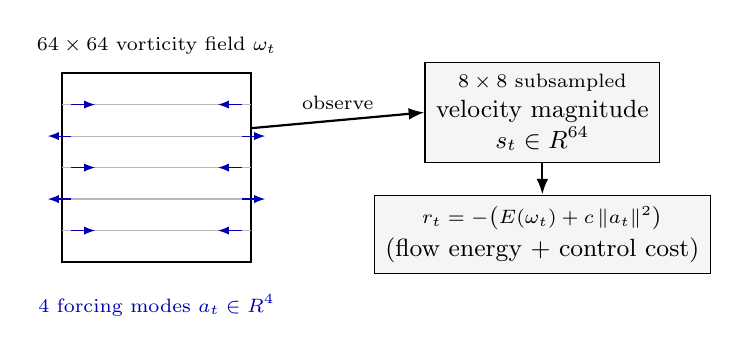
\begin{tikzpicture}[node distance=6mm]
  % flow domain
  \draw[thick] (0,0) rectangle (2.4,2.4);
  \foreach \y in {0.4,0.8,1.2,1.6,2.0}{\draw[gray!55] (0,\y) -- (2.4,\y);}
  \node[font=\scriptsize] at (1.2,2.75) {$64\times 64$ vorticity field $\omega_t$};
  % actuator arrows (sinusoidal forcing modes)
  \foreach \y/\s in {0.4/0.3,0.8/-0.3,1.2/0.3,1.6/-0.3,2.0/0.3}{
    \draw[-{Latex[length=1.4mm]},blue!70!black] (0.12,\y) -- ($(0.12,\y)+(\s,0)$);
    \draw[-{Latex[length=1.4mm]},blue!70!black] (2.28,\y) -- ($(2.28,\y)-(\s,0)$);}
  \node[blue!70!black,font=\scriptsize] at (1.2,-0.55)
    {4 forcing modes $a_t\in\mathbb{R}^4$};

  % observation
  \node[databox,align=center] (obs) at (6.1,1.9)
    {\scriptsize $8\times 8$ subsampled\\ velocity magnitude\\ $s_t\in\mathbb{R}^{64}$};
  \draw[flow] (2.4,1.7) -- (obs.west) node[midway,above,font=\scriptsize]{observe};

  % reward
  \node[databox,align=center] (rew) at (6.1,0.35)
    {\scriptsize $r_t = -\big(E(\omega_t)+c\,\lVert a_t\rVert^2\big)$\\[1pt]
     (flow energy $+$ control cost)};
  \draw[flow] (obs.south) -- (rew.north);
\end{tikzpicture}
\caption{Kolmogorov-flow control problem. The policy observes an $8\times 8$
subsampled velocity magnitude ($s_t\in\mathbb{R}^{64}$), commands four
sinusoidal forcing-mode amplitudes ($a_t\in\mathbb{R}^{4}$), and is rewarded
for reducing flow energy at bounded control cost. The library default
$\alpha_{\text{reward}}=0$ (control-cost only) is overridden to
$\alpha_{\text{reward}}=1$ so that flow energy enters the reward.}
\label{fig:env}
\end{figure*}

Two library quirks required a subclass. (i) The environment step ignores the
per-call time-step and action-duration arguments and re-reads its own
\texttt{default\_params}, so we override that property on a subclass
(\texttt{FastKolmogorovFlow}) to reach proof-of-concept scale.
(ii) The library default $\alpha_{\text{reward}}=0$ makes the reward
control-cost only; we set $\alpha_{\text{reward}}=1$ (\cref{fig:env}).

At this grid/$\dd t$ combination ($64\times 64$, $\dd t=0.001$) the solver was
empirically observed to diverge numerically near $\Re\approx 350$--$380$ ---
even under zero action from purely analytic initial conditions, and not
resolved by reducing $\dd t$ tenfold (so not a simple CFL issue). We
therefore use $\Re=300$ for the chaotic regime --- the highest value that
stays below this limit while forming a meaningful contrast with $\Re=45$ ---
rather than the originally intended $\Re=450$.

\subsection{Markov decision process}
\label{sec:mdp}

The control task is a Markov decision process
$(\mathcal{S},\mathcal{A},P,r,\gamma)$ with
$s_t\in\mathbb{R}^{64}$, $a_t\in\mathbb{R}^{4}$, deterministic transition
$s_{t+1}=g\big(f_{\mathrm{sim}}(\omega_t,a_t;\Re)\big)$ ($g$ the observation
map), reward as in \cref{fig:env}, and discount $\gamma=0.99$. An episode is
$T=15$ environment steps from a fixed reset state $s_0$. The policy
$\pi_\theta(a\mid s)$ and the value / $Q$ networks are 2-hidden-layer MLPs
(64 units, $\tanh$). The objective is the discounted return
\begin{equation}
  J(\theta)=\mathbb{E}_{\tau\sim\pi_\theta}\!\left[\textstyle\sum_{t=0}^{T-1}\gamma^{t}\,r(s_t,a_t)\right].
  \label{eq:return}
\end{equation}
All four algorithms optimize \cref{eq:return}; they differ only in the
gradient estimator they apply to it.

\subsection{PPO: on-policy baseline}
\label{sec:ppo}

PPO is an on-policy policy-gradient method: it collects one rollout under
the current policy, estimates each action's advantage along it, and takes a
single trust-region-style step that is clipped to stay close to the policy
that generated the data. The rollout is then discarded, so PPO consumes
each unit of environment experience through exactly one gradient update.

The clipped surrogate is due to Schulman et al.\ as a first-order
approximation to the TRPO trust region~\cite{ppo2017,trpo2015}, and the
Generalized Advantage Estimator (GAE) used to form the advantage is from the
same group~\cite{gae2015}. All gradient steps in this study, for every
algorithm, use Adam~\cite{kingma2015adam}, as in the original PPO and
HydroGym~\cite{hydrogym2026} implementations.

The policy is a diagonal Gaussian: the MLP produces a bounded mean
$a_{\mu}(s)=0.5\tanh(\cdot)$ and a state-independent learnable
$\log\sigma$; the executed action is $a\sim\mathcal{N}(a_\mu(s),\sigma^2)$
and is \emph{not} re-clipped, so sampled $\lvert a\rvert$ can exceed
$0.5$ (observed up to $\approx 1.2$ early in training). Advantages use
GAE~\cite{gae2015}:
\begin{equation}
  \hat{A}_t=\sum_{l=0}^{T-t-1}(\gamma\lambda)^{l}\delta_{t+l},\qquad
  \delta_t=r_t+\gamma V(s_{t+1})-V(s_t),
  \label{eq:gae}
\end{equation}
with $\lambda=0.95$. PPO maximizes the clipped
surrogate~\cite{ppo2017}, derived from the TRPO trust
region~\cite{trpo2015}:
\begin{equation}
  \begin{split}
    \mathcal{L}^{\mathrm{PPO}}(\theta)&=\mathbb{E}_t\!\Big[\min\!\big(\rho_t(\theta)\hat{A}_t,\\
    &\qquad \mathrm{clip}(\rho_t(\theta),1-\epsilon,1+\epsilon)\hat{A}_t\big)\Big],\\
    \rho_t(\theta)&=\frac{\pi_\theta(a_t\mid s_t)}{\pi_{\theta_{\text{old}}}(a_t\mid s_t)},
  \end{split}
  \label{eq:ppo}
\end{equation}
with $\epsilon=0.2$. The total loss adds a value term and an entropy bonus,
\begin{equation}
  \begin{split}
    \mathcal{L}&=-\mathcal{L}^{\mathrm{PPO}}+0.5\,\mathcal{L}^{V}-0.001\,\mathcal{H}[\pi_\theta],\\
    \mathcal{L}^{V}&=\mathbb{E}_t\big[(V_\phi(s_t)-\hat{R}_t)^2\big].
  \end{split}
  \label{eq:ppoloss}
\end{equation}

Our loop performs \emph{one
full-batch gradient step per episode} on \cref{eq:ppoloss} --- no PPO
epochs, no minibatching. This is a deliberately minimal PPO: it keeps the
on- and off-policy loops comparable and the analytic-gradient mix simple,
but ``PPO'' here is weaker than a fully tuned implementation. The comparison
of interest is relative (PPO vs.\ GPPO, SAC vs.\ GSAC), and all four share
this budget.

We use PPO as the on-policy baseline, rather than a
different on-policy algorithm, because it is exactly the update the
HydroGym paper's GPPO result is built on top of~\cite{hydrogym2026}:
answering whether that result survives a chaotic regime requires holding
the base update fixed and changing only the analytic-gradient mixing
(\cref{sec:gppo}), not also switching algorithms. Its clipped surrogate also
gives a clean model-free-only control arm for the on-policy row of the
$2\times 2$ design (\cref{fig:design}).

\subsection{SAC: off-policy baseline}
\label{sec:sac}

SAC is an off-policy, maximum-entropy actor-critic method: transitions are
stored in a replay buffer and resampled many times, so one environment step
contributes to many gradient updates instead of one. Its actor is a
squashed Gaussian whose action is drawn by reparameterized sampling, so the
entropy-regularized objective can be differentiated through the sampled
action directly rather than estimated by a likelihood-ratio term.

SAC and its maximum-entropy objective are due to Haarnoja et
al.~\cite{sac2018,sacapps2018}, building on Soft
Q-learning~\cite{softq2017}; its twin critics adopt the overestimation-bias
fix introduced for off-policy actor-critic methods by
TD3~\cite{fujimoto2018td3}, and the reparameterized actor gradient traces to
the stochastic backpropagation of Rezende et
al.~\cite{rezende2014stochastic}, the same mechanism used earlier for
deterministic actors in DDPG~\cite{lillicrap2016ddpg}. SAC uses twin
$Q$-critics $Q_{\psi_1},Q_{\psi_2}$ and target networks to optimize:
\begin{equation}
  J_{\mathrm{ME}}(\pi)=\mathbb{E}\!\left[\textstyle\sum_t r(s_t,a_t)+\alpha\,\mathcal{H}\!\big(\pi(\cdot\mid s_t)\big)\right],
  \label{eq:sacobj}
\end{equation}
with fixed temperature $\alpha=0.1$ (not auto-tuned). The actor and critic
losses are
\begin{align}
  J_\pi(\varphi)     &=\mathbb{E}_{s\sim\mathcal{D},\,a\sim\pi_\varphi}\!\big[\alpha\log\pi_\varphi(a\mid s)-\min_i Q_{\psi_i}(s,a)\big],
  \label{eq:sacactor}\\
  J_Q(\psi_i)        &=\mathbb{E}_{(s,a,r,s')\sim\mathcal{D}}\!\Big[\big(Q_{\psi_i}(s,a)-y\big)^2\Big],\\
  y&=r+\gamma\big(\min_j Q_{\bar\psi_j}(s',a')-\alpha\log\pi_\varphi(a'\mid s')\big),
  \label{eq:saccritic}
\end{align}
with soft target updates
$\bar\psi_i\leftarrow(1-\tau_s)\bar\psi_i+\tau_s\psi_i$, $\tau_s=0.005$. Per
episode, the rollout's 15 transitions are added to a replay buffer $\mathcal{D}$
(capacity $=n_{\text{ep}}\times 15$) and 10 gradient updates are performed
with batch size 64.

SAC is the natural off-policy counterpart to PPO
along exactly the factor this study varies (\cref{fig:design}): both
optimize a stochastic policy with an actor-critic architecture, so replacing
PPO's rollout-and-discard loop with SAC's replay buffer isolates the
on-/off-policy factor without also changing the policy family, as switching
to a deterministic actor (DDPG/TD3) would. Its replay buffer also gives the
off-policy family a mechanism, buffer dilution, that PPO structurally lacks;
\cref{sec:buffer} uses this to explain why on-policy and off-policy runs can
behave differently immediately after a chaotic-regime trigger episode even
when neither family is more failure-prone on average. We sample the buffer
uniformly rather than by TD-error priority~\cite{schaul2016per}, so that any
such difference is attributable to the on-/off-policy structure itself and
not to a secondary sampling scheme.

\subsection{Analytic policy gradient}
\label{sec:analytic}

The analytic gradient is the derivative of a short rollout's accumulated
reward with respect to the policy parameters, obtained by unrolling the
policy's \emph{deterministic mean} action through the differentiable solver
and differentiating end-to-end with reverse-mode automatic differentiation.
It is a low-variance but biased estimator, so its length is capped at
$H=6$ steps and it is mixed with the model-free gradient at a fixed 50/50
weight rather than trusted alone (\cref{fig:analytic}).

Backpropagating through a rollout is the classical
backpropagation-through-time construction~\cite{werbos1990bptt}; SHAC~\cite{shac2022}
and AHAC~\cite{ahac2024} apply the same short-horizon truncation to
differentiable simulators, and Metz et al.~\cite{metz2021} and Parmas et
al.~\cite{parmas2018pipps} show that such backpropagated gradients can
explode and lose direction under chaotic dynamics. Over $H=6$ steps we
forward-propagate the policy's mean action (no sampling, so the whole chain
stays smooth) and differentiate the negative accumulated reward:
\begin{equation}
  \begin{split}
    \Lan(\theta)&=-\sum_{t=1}^{H}r\big(s_t,a_\mu(s_t;\theta)\big),\\
    s_t&=f_{\mathrm{sim}}(s_{t-1},a_\mu(s_{t-1};\theta);\Re),\\
    \gan&=\nabla_\theta\Lan(\theta),
  \end{split}
  \label{eq:analytic}
\end{equation}
computed by \texttt{jax.grad}. The final gradient mixes $\gan$ with the
model-free gradient $g_{\mathrm{mf}}\in\{g_{\mathrm{PPO}},g_\pi\}$ at equal
weight:
\begin{equation}
  g_{\mathrm{final}}=\beta\,\gan+(1-\beta)\,g_{\mathrm{mf}},\qquad \beta=0.5,
  \label{eq:mix}
\end{equation}
the $\alpha=0.5$ special case of the $\alpha$-graded estimator of Suh et
al.~\cite{suh2022}, of the total-gradient decomposition of Parmas and
Sugiyama~\cite{parmas2018total}, and the non-adaptive limit of the GI-PPO
$\alpha$-policy~\cite{gippo2023}. \Cref{eq:mix} is the only structural
difference between PPO and GPPO, and between SAC and GSAC.

\begin{figure*}[t]
\centering
\resizebox{\textwidth}{!}{%
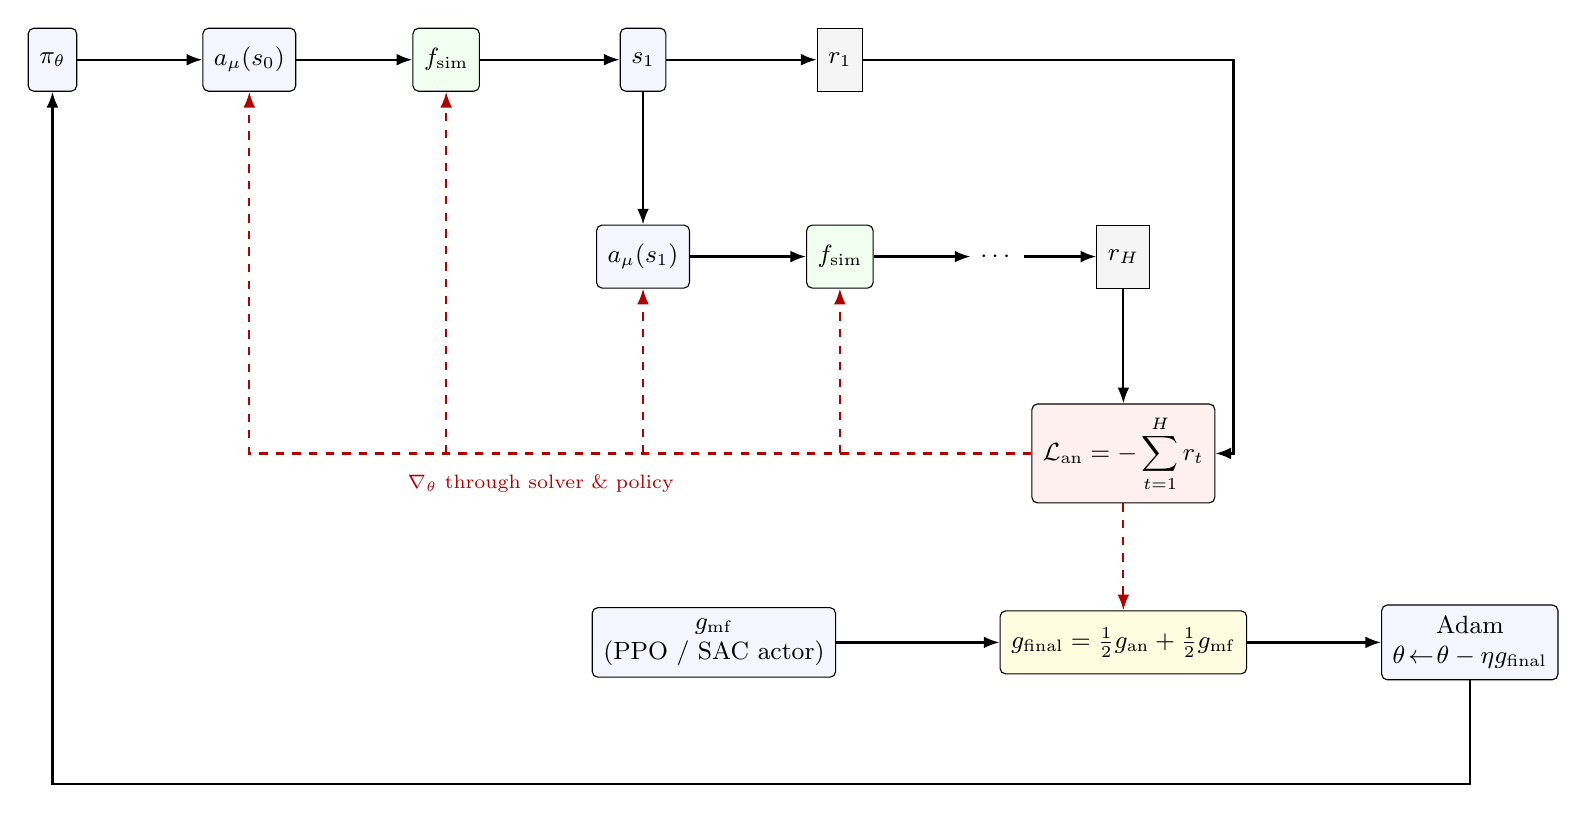
\begin{tikzpicture}
  % forward rollout, row 1
  \node[block] (pi0) at (0,0) {$\pi_\theta$};
  \node[block] (a1)  at (2.5,0) {$a_\mu(s_0)$};
  \node[envblock] (f1) at (5.0,0) {$f_{\mathrm{sim}}$};
  \node[block] (s1)  at (7.5,0) {$s_1$};
  \node[databox] (r1) at (10.0,0) {$r_1$};
  % forward rollout, row 2
  \node[block] (a2)  at (7.5,-2.5) {$a_\mu(s_1)$};
  \node[envblock] (f2) at (10.0,-2.5) {$f_{\mathrm{sim}}$};
  \node[font=\small] (dots) at (12.0,-2.5) {$\cdots$};
  \node[databox] (rH) at (13.6,-2.5) {$r_H$};
  \node[anblock] (L) at (13.6,-5.0) {$\displaystyle \Lan=-\sum_{t=1}^{H}r_t$};

  \draw[flow] (pi0)--(a1); \draw[flow] (a1)--(f1); \draw[flow] (f1)--(s1);
  \draw[flow] (s1)--(r1);
  \draw[flow] (s1)--(a2);
  \draw[flow] (a2)--(f2); \draw[flow] (f2)--(dots); \draw[flow] (dots)--(rH);
  \draw[flow] (rH)--(L);
  \draw[flow] (r1.east) -- (15.0,0) -- (15.0,-5.0) -- (L.east);

  % backward analytic gradient: one bus under the rollout, orthogonal drops
  \draw[grad] (L.west) -- (2.5,-5.0) -- (a1.south);
  \draw[grad] (5.0,-5.0) -- (f1.south);
  \draw[grad] (7.5,-5.0) -- (a2.south);
  \draw[grad] (10.0,-5.0) -- (f2.south);
  \node[font=\scriptsize,text=red!70!black,anchor=north] at (6.2,-5.15)
    {$\nabla_\theta$ through solver \& policy};

  % mixer and optimiser
  \node[block,fill=yellow!12] (mix) at (13.6,-7.4)
    {$g_{\mathrm{final}}=\tfrac12\gan+\tfrac12 g_{\mathrm{mf}}$};
  \node[block] (mf) at (8.4,-7.4) {$g_{\mathrm{mf}}$\\(PPO / SAC actor)};
  \node[block] (adam) at (18.0,-7.4) {Adam\\ $\theta\!\leftarrow\!\theta-\eta g_{\mathrm{final}}$};
  \draw[grad] (L) -- (mix);
  \draw[flow] (mf) -- (mix);
  \draw[flow] (mix) -- (adam);
  \draw[flow] (adam.south) -- (18.0,-9.2) -- (0,-9.2) -- (pi0.south);
\end{tikzpicture}}
\caption{Analytic-gradient computation graph (\cref{eq:analytic,eq:mix}).
Solid arrows: forward rollout of the \emph{deterministic mean} action
through the differentiable solver for $H=6$ steps. Dashed red arrows:
reverse-mode differentiation of the accumulated reward $\Lan$ with respect to
$\theta$ via \texttt{jax.grad}. The analytic gradient is averaged 50/50 with
the model-free gradient and applied with Adam. Replacing the mixer with
$g_{\mathrm{final}}=g_{\mathrm{mf}}$ recovers plain PPO / SAC.}
\label{fig:analytic}
\end{figure*}

We fix $\beta=0.5$ and $H=6$
rather than adapting either online, because this study asks whether
analytic-gradient injection helps or hurts as the regime turns chaotic, and
an adaptive scheme such as GI-PPO's $\alpha$-policy or SAPO's entropy-based
smoothing would let the algorithm partially opt out of the analytic term
exactly when the chaotic regime makes it unreliable --- confounding the
effect under test. \Cref{sec:gppo,sec:gsac} apply this same fixed rule to
the on-policy and off-policy actor gradient respectively, so that GPPO and
GSAC differ from PPO and SAC by exactly one mechanism.

\subsection{GPPO: on-policy variant}
\label{sec:gppo}

GPPO adds the analytic-gradient mix of \cref{eq:mix} to the PPO update: from
the same fixed reset state, a deterministic $H=6$-step analytic rollout runs
alongside the standard stochastic on-policy rollout, and the two resulting
gradients are averaged before a single Adam step (\cref{fig:gppo,alg:gppo}).
Every other setting --- rollout length, GAE, the clip range, network
architecture, and learning rate --- is identical to plain PPO (\cref{sec:ppo}).

This is the same mechanism as the HydroGym paper's GPPO, reported to cut
training iterations by at least \SI{65}{\percent} over PPO on Kolmogorov
flow~\cite{hydrogym2026}. That paper does not report its horizon length or
mixing weight, so ours follow the general short-horizon-and-mix recipe of
SHAC, AHAC, and GI-PPO (\cref{sec:analytic}) rather than an attempt to match
unpublished hyperparameters.

\begin{figure*}[t]
\centering
\resizebox{\textwidth}{!}{%
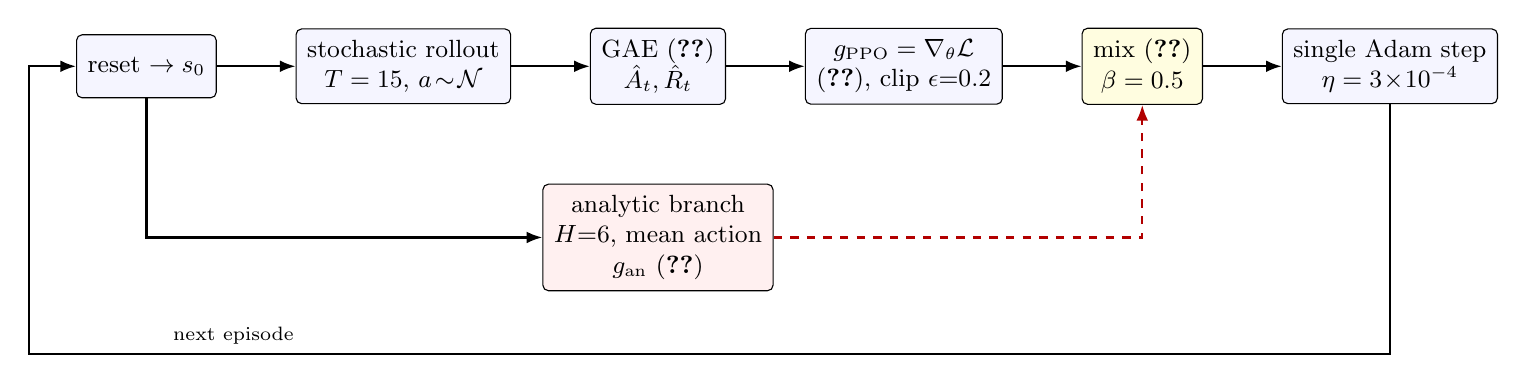
\begin{tikzpicture}[node distance=6mm and 10mm]
  \node[block] (reset) {reset $\to s_0$};
  \node[block,right=of reset] (roll) {stochastic rollout\\ $T=15$, $a\!\sim\!\mathcal{N}$};
  \node[block,right=of roll] (gae) {GAE \eqref{eq:gae}\\ $\hat A_t,\hat R_t$};
  \node[block,right=of gae] (gppo) {$g_{\mathrm{PPO}}=\nabla_\theta\mathcal{L}$\\ \eqref{eq:ppoloss}, clip $\epsilon{=}0.2$};
  \node[block,right=of gppo,fill=yellow!12] (mix) {mix \eqref{eq:mix}\\ $\beta=0.5$};
  \node[block,right=of mix] (adam) {single Adam step\\ $\eta=3\!\times\!10^{-4}$};
  \node[anblock,below=10mm of gae] (an) {analytic branch\\ $H{=}6$, mean action\\ $\gan$ \eqref{eq:analytic}};
  \draw[flow] (reset)--(roll); \draw[flow] (roll)--(gae); \draw[flow] (gae)--(gppo);
  \draw[flow] (gppo)--(mix); \draw[flow] (mix)--(adam);
  \draw[flow] (reset.south) |- (an.west);
  \draw[grad] (an.east) -| (mix.south);
  % next episode: below everything, re-enter reset from the left
  \coordinate (low) at ($(an.south)+(0,-8mm)$);
  \draw[flow] (adam.south) -- (adam.south |- low) -- ($(reset.west |- low)+(-6mm,0)$)
      -- ($(reset.west)+(-6mm,0)$) -- (reset.west);
  \node[font=\scriptsize,above,anchor=south] at ($(reset.west |- low)+(2cm,0)$) {next episode};
\end{tikzpicture}}
\caption{GPPO training loop (one episode). The analytic branch is a
deterministic 6-step unroll that runs in parallel with the standard on-policy
update; the two gradients are averaged before a single Adam step. Removing
the red branch gives PPO.}
\label{fig:gppo}
\end{figure*}

\begin{algorithm}[t]
\caption{GPPO --- one training episode ($\beta=0.5$, $H=6$)}
\label{alg:gppo}
\DontPrintSemicolon
\KwIn{policy $\theta$, value $\phi$, optimizer state, fixed reset state $s_0$}
$\tau \leftarrow \textproc{rollout}(\pi_\theta, s_0)$ for $T=15$ steps
  \tcp*{sample $a_t\sim\mathcal{N}(a_\mu(s_t),\sigma^2)$}
$\hat A,\hat R \leftarrow \textproc{GAE}(\tau;\gamma{=}0.99,\lambda{=}0.95)$\;
$g_{\mathrm{PPO}} \leftarrow \nabla_\theta\big[-\mathcal{L}^{\mathrm{PPO}}(\theta;\tau,\hat A)+0.5\,\mathcal{L}^{V}(\phi;\tau,\hat R)-0.001\,\mathcal{H}(\pi_\theta)\big]$\;
\tcp{analytic branch: deterministic, differentiable, short horizon}
$\Lan(\theta) \leftarrow -\sum_{t=1}^{H} r\big(f_{\mathrm{sim}}^{\,t}(s_0,a_\mu(\cdot\,;\theta))\big)$\;
$\gan \leftarrow \nabla_\theta \Lan(\theta)$ \tcp*{\texttt{jax.grad} through the solver}
$g \leftarrow \beta\,\gan + (1-\beta)\,g_{\mathrm{PPO}}$\;
$\theta \leftarrow \textproc{Adam}(\theta, g;\ \eta{=}3\!\times\!10^{-4})$ \tcp*{single full-batch step}
\KwOut{$\theta,\phi$; \; logs $\big(\lVert\gan\rVert,\ \mathrm{RMS}\lvert a_t\rvert,\ \max\lvert a_t\rvert,\ \sum_t r_t\big)$}
PPO is this algorithm with the analytic branch (the $\Lan$, $\gan$, and mixing steps) removed, so that $g \leftarrow g_{\mathrm{PPO}}$.
\end{algorithm}

GPPO is the on-policy arm of the $2\times 2$
design and the direct object of the reproduction question this paper asks:
does the reported sample-efficiency gain hold, under the same fixed recipe,
at a chaotic operating point where the analytic gradient's premises ---
smooth, low-variance backpropagation through the solver --- are not
expected to hold? \cref{sec:results} answers this at $\Re=45$ (yes) and
$\Re=300$ (no seed-robust effect).

\subsection{GSAC: off-policy variant}
\label{sec:gsac}

GSAC applies the same analytic-gradient mix to the SAC actor rather than to
PPO's surrogate: after each episode's rollout and ten off-policy
critic-and-actor updates, one further actor step mixes the last actor
gradient, $g_{\mathrm{mf}}=g_\pi=\nabla_\varphi J_\pi(\varphi)$ from
\cref{eq:sacactor}, with a deterministic $H=6$-step analytic rollout from
the reset state (\cref{fig:gsac,alg:gsac}). The critics, target networks,
and replay mechanics are otherwise unchanged from plain SAC (\cref{sec:sac}).

This follows SAPO's core motivation of combining an off-policy,
maximum-entropy actor with an analytic gradient~\cite{sapo2025}, but
targets HydroGym's Kolmogorov flow rather than SAPO's rigid/deformable-body
platform, and uses the same fixed 50/50 mix as GPPO (\cref{sec:analytic})
rather than SAPO's entropy-based smoothing. To our knowledge this is the
first application of an off-policy, maximum-entropy analytic-gradient
method to a fluid-dynamics control task.

\begin{figure*}[t]
\centering
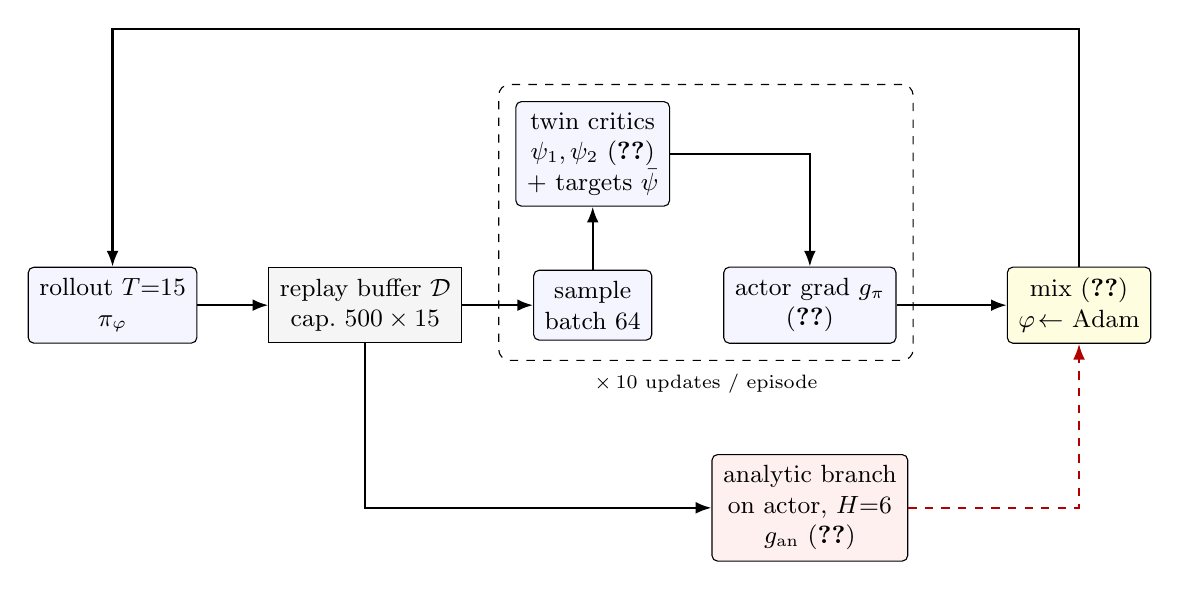
\begin{tikzpicture}[node distance=6mm and 9mm]
  \node[block] (roll) {rollout $T{=}15$\\ $\pi_\varphi$};
  \node[databox,right=of roll] (buf) {replay buffer $\mathcal{D}$\\ cap.\ $500\times 15$};
  \node[block,right=of buf] (batch) {sample\\ batch 64};
  \node[block,above=8mm of batch] (crit) {twin critics\\ $\psi_1,\psi_2$ \eqref{eq:saccritic}\\ $+$ targets $\bar\psi$};
  \node[block,right=of batch] (act) {actor grad $g_\pi$\\ \eqref{eq:sacactor}};
  \node[draw,dashed,rounded corners,fit=(batch)(crit)(act),inner sep=6pt] (inner) {};
  \node[font=\scriptsize,anchor=north] at ($(inner.south)+(0,-1pt)$) {$\times\,10$ updates / episode};
  \node[anblock,below=14mm of act] (an) {analytic branch\\ on actor, $H{=}6$\\ $\gan$ \eqref{eq:analytic}};
  \node[block,right=14mm of act,fill=yellow!12] (mix) {mix \eqref{eq:mix}\\ $\varphi\!\leftarrow$ Adam};
  \coordinate (top) at ($(inner.north)+(0,7mm)$);
  \draw[flow] (roll)--(buf); \draw[flow] (buf)--(batch);
  \draw[flow] (batch)--(crit); \draw[flow] (crit.east) -| (act.north);
  \draw[flow] (act.east) -- (mix.west);
  \draw[grad] (an.east) -| (mix.south);
  \draw[flow] (buf.south) |- (an.west);
  \draw[flow] (mix.north) -- (mix.north |- top) -- (roll.north |- top) -- (roll.north);
\end{tikzpicture}
\caption{GSAC training loop (one episode). Ten off-policy critic$+$actor
updates on replay batches are followed by a single analytic actor step
(6-step deterministic unroll from the reset state). Removing the red branch
and the mixer gives SAC.}
\label{fig:gsac}
\end{figure*}

\begin{algorithm}[t]
\caption{GSAC --- one training episode ($\beta=0.5$, $H=6$)}
\label{alg:gsac}
\DontPrintSemicolon
\KwIn{actor $\varphi$, critics $\psi_1,\psi_2$, targets $\bar\psi_1,\bar\psi_2$, replay buffer $\mathcal{D}$, reset state $s_0$}
$\tau \leftarrow \textproc{rollout}(\pi_\varphi, s_0)$ for $T=15$ steps;\quad $\mathcal{D} \leftarrow \mathcal{D}\cup\tau$\;
\For{$k = 1 \ldots 10$}{
  $B \leftarrow \textproc{sample}(\mathcal{D}, 64)$\;
  \lFor{$i\in\{1,2\}$}{$\psi_i \leftarrow \textproc{Adam}\big(\psi_i, \nabla_{\psi_i} J_Q(\psi_i; B)\big)$}
  $g_\pi \leftarrow \nabla_\varphi\,\mathbb{E}_{s\in B}\big[\alpha\log\pi_\varphi(a\mid s)-\min_i Q_{\psi_i}(s,a)\big],\ a\sim\pi_\varphi(\cdot\mid s),\ \alpha=0.1$\;
  $\varphi \leftarrow \textproc{Adam}(\varphi, g_\pi)$\;
  $\bar\psi_i \leftarrow (1-\tau_s)\bar\psi_i + \tau_s\psi_i,\quad \tau_s=0.005$\;
}
\tcp{analytic branch on the actor, after the SAC updates}
$\gan \leftarrow \nabla_\varphi\big[-\sum_{t=1}^{H} r\big(f_{\mathrm{sim}}^{\,t}(s_0,a_\mu(\cdot\,;\varphi))\big)\big]$\;
$\varphi \leftarrow \textproc{Adam}\big(\varphi,\ \beta\,\gan + (1-\beta)\,g_\pi\big)$ \tcp*{$g_\pi$ from the last inner step}
\KwOut{$\varphi,\psi$; \; logs $\big(\lVert\gan\rVert,\ \mathrm{RMS}\lvert a_t\rvert,\ \max\lvert a_t\rvert,\ \sum_t r_t\big)$}
SAC is this algorithm with the analytic branch (the final $\gan$ and mixing steps) removed.
\end{algorithm}

GSAC completes the $2\times 2$ design
(\cref{fig:design}) and lets this study ask its second question directly:
does an off-policy replay buffer tolerate the analytic gradient's
chaotic-regime instability better than an on-policy rollout, or does adding
a replay buffer simply add its own failure mode? Because GPPO and GSAC
share the identical analytic branch (\cref{eq:analytic}) and mixing rule
(\cref{eq:mix}), any difference in chaotic-regime robustness between them is
attributable to the on-/off-policy factor rather than to a different
analytic-gradient implementation.

GAE, PPO clipping, and the 50/50
analytic/model-free mix are hand-rolled in plain JAX/optax and kept
identical in form across the PPO and SAC training scripts. Both scripts
additionally log per-episode action amplitude (RMS and absolute max) for the
trigger-episode diagnostic of \cref{sec:mechanism}.

\section{Experimental setup and reproducibility}
\label{sec:setup}

\subsection{Configuration}

\Cref{tab:config} lists every hyperparameter. All four algorithms are trained
for \num{500} episodes at both Reynolds numbers, matching the training budget
reported by the HydroGym paper~\cite{hydrogym2026}.

\begin{table*}[t]
\centering
\caption{Full configuration. Identical across all four algorithms except
where an algorithm-specific row applies.}
\label{tab:config}
\small
\setlength{\tabcolsep}{4pt}
\resizebox{\textwidth}{!}{%
\begin{tabular}{|l|l|}
\hline
Parameter & Value \\
\hline
Grid & $64\times 64$ (4096 DOF) \\
\hline
Solver & pseudo-spectral IMEX-RK4CN (real \texttt{hydrogym.jax}) \\
\hline
$\Re$ (regular / chaotic) & 45 / 300 \\
\hline
Episodes / steps per episode & 500 / 15 \\
\hline
Environment $\dd t$ / \texttt{action\_time} & 0.001 / 1.0 \\
\hline
Reward & $\alpha_{\text{reward}}=1$ (flow energy $+$ control cost) \\
\hline
Analytic horizon (GPPO/GSAC) & $H=6$ steps, mean (deterministic) action \\
\hline
Gradient mixing & $0.5\cdot$ model-free $+\ 0.5\cdot$ analytic \\
\hline
Optimizer / learning rate & Adam / $3\times 10^{-4}$ (actor and critic) \\
\hline
Policy / value / critic network & 2 hidden layers $\times$ 64 units, $\tanh$ \\
\hline
Action & PPO: $a_\mu=0.5\tanh(\cdot)$, sampled, not re-clipped;\\
       & SAC: squashed $\tanh$ \\
\hline
PPO & $\gamma{=}0.99$, $\lambda{=}0.95$, clip $\epsilon{=}0.2$, entropy coeff.\ 0.001,\\
    & 1 full-batch step / episode \\
\hline
SAC & $\gamma{=}0.99$, $\alpha{=}0.1$ (fixed), $\tau_s{=}0.005$,\\
    & 10 updates / episode, batch 64, buffer $= 500\times 15$ \\
\hline
Seeds & $n=5$ (seed $=0$--$4$) \\
\hline
Hardware & RTX 5060 laptop GPU (8\,GB), JAX 0.10.2 $+$ CUDA 12 \\
\hline
\end{tabular}%
}

\end{table*}

\subsection{Seed protocol}
\label{sec:seedprotocol}

Each $(\text{algorithm},\Re,\text{seed})$ triple is trained independently for
five seeds. The JAX PRNG is fully deterministic, so a given
$(\text{config},\text{seed})$ is bit-for-bit reproducible --- the
$\text{seed}=3$ GSAC/$\Re=300$ run was regenerated identically after its first
dump was lost. Configurations are run strictly one at a time: this class of
consumer GPU cannot host concurrent JAX processes without severe memory
contention. Per-seed wall time for the full 8-configuration sweep is
$\sim$6--8.5\,h ($\text{seed}=4$: $\sim$6.2\,h; PPO $\sim$28\,min/config,
GPPO $\sim$63\,min, SAC $\sim$28\,min, GSAC $\sim$60\,min).

\subsection{Reproducibility package}

Following the ML reproducibility checklist~\cite{pineau2021}, the release
will include the experiment code as a standalone repository separated from
the upstream HydroGym clone; a pinned environment specification (122
packages), a portable environment-rebuild script, and the parametrized sweep
driver; every per-configuration result dump --- episode rewards,
analytic-gradient norms, action-amplitude logs, and wall times --- together
with the driver logs; and a Zenodo DOI accompanied by ``Code availability''
and ``Data availability'' statements.

\subsection{Analysis of the chaotic-regime outcome}
\label{sec:analysisplan}

The outcome variable at $\Re=300$ is the \emph{first-NaN episode} --- the
training episode at which the flow simulation first returns a non-finite
reward. This is not a short-circuit: training continues to run all 500
episodes regardless. The four algorithms are compared pairwise on their five
paired per-seed differences using an exact sign-flip permutation
test (all $2^5=32$ relabelings, two-sided) and a bootstrap
\SI{95}{\percent} CI for the median difference (\num{20000} resamples).
Omnibus tests are Kruskal--Wallis (unblocked) and Friedman (blocked by
seed). The pre-registered decision rule (\cref{sec:intro}): report ``no
seed-robust ordering'' unless GSAC beats every other algorithm at
$p<0.05$ one-sided.

\section{Results}
\label{sec:results}

\subsection{Regular regime ($\Re=45$): sample efficiency}
\label{sec:re45}

At $\Re=45$, GPPO reaches PPO's best 500-episode smoothed reward in
substantially fewer episodes in 4 of 5 seeds ($\text{seed}=0$:
\SI{63}{\percent} fewer; $\text{seed}=1$: $\sim$\SI{78}{\percent};
$\text{seed}=3$: $\sim$\SI{84}{\percent}; $\text{seed}=4$:
$\sim$\SI{70}{\percent}), and by a smaller margin at $\text{seed}=2$
($\sim$\SI{26}{\percent}). The \emph{direction} of GPPO's advantage over PPO
holds in all five seeds, and the $\text{seed}=0$ value (\SI{63}{\percent}) is
close to the paper's reported \SI{65}{\percent}~\cite{hydrogym2026} ---
evidence that our reimplementation captures the paper's mechanism.
\Cref{fig:re45curves} shows the seed-averaged learning curves.

\begin{figure}[t]
\centering
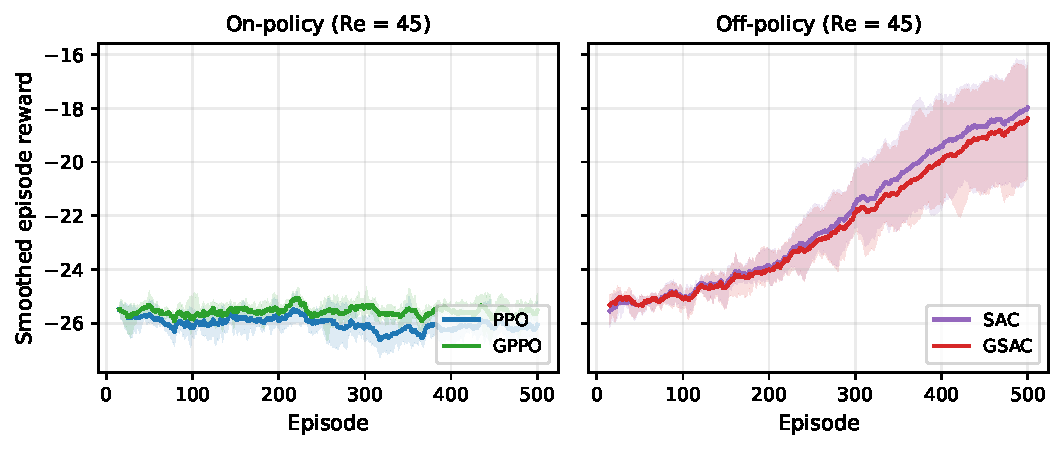
\includegraphics[width=\linewidth]{fig_re45_curves.pdf}
\caption{Regular regime ($\Re=45$). Seed-averaged smoothed episode reward
(15-episode window); shaded band is the seed-wise min--max envelope over the
five seeds. The off-policy family (right) converges to a markedly higher
reward level than the on-policy family (left); within each family the
analytic-gradient variant tracks its base algorithm closely.}
\label{fig:re45curves}
\end{figure}

\begin{figure}[tbp]
\centering
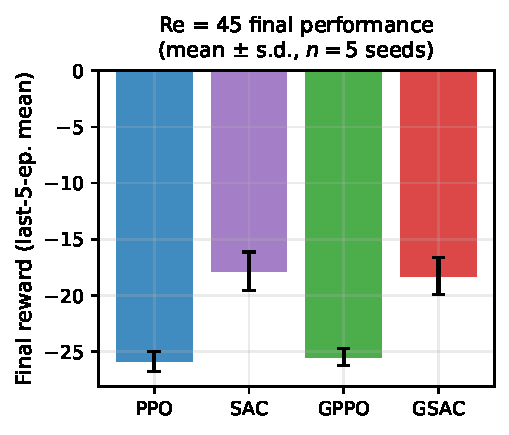
\includegraphics[width=0.6\linewidth]{fig_re45_final.pdf}
\caption{Final reward at $\Re=45$ (last-5-episode mean, mean $\pm$ s.d.\ over
five seeds). SAC/GSAC clearly outperform PPO/GPPO; GSAC does not exceed SAC.}
\label{fig:re45final}
\end{figure}

Two $\Re=45$ findings are seed-stable (\cref{fig:re45final}): (i) the
off-policy family reaches clearly better final reward than the on-policy
family in every seed --- its replay-buffer structure is already far more
sample-efficient, so no GPPO-style acceleration analysis applies to it; and
(ii) GSAC does not exceed SAC's final performance in any seed --- the
analytic gradient does not help the off-policy method in the regular regime.

\begin{table}[tbp]
\centering
\caption{Final performance at $\Re=45$, last-5-episode mean reward
(seed $=0\,/\,1\,/\,2\,/\,3\,/\,4$).}
\label{tab:re45}
\small
\begin{tabular}{|l|l|}
\hline
Algorithm & Final reward \\
\hline
PPO  & $-25.1\,/\,{-25.2}\,/\,{-27.2}\,/\,{-26.4}\,/\,{-25.6}$ \\
\hline
GPPO & $-25.4\,/\,{-24.6}\,/\,{-26.7}\,/\,{-25.4}\,/\,{-25.4}$ \\
\hline
SAC  & $-16.7\,/\,{-16.9}\,/\,{-18.9}\,/\,{-16.3}\,/\,{-20.3}$ \\
\hline
GSAC & $-18.0\,/\,{-17.1}\,/\,{-20.4}\,/\,{-16.3}\,/\,{-19.5}$ \\
\hline
\end{tabular}
\end{table}

\Cref{tab:re45} gives the exact per-seed values underlying \cref{fig:re45final}.
$\text{seed}=2$ trained to a worse level across all four algorithms, but the
\emph{relative} ordering is unchanged.

\subsection{Chaotic regime ($\Re=300$): the breaking point has no stable ordering}
\label{sec:re300}

In the chaotic regime all four algorithms have a breaking point ---
none completes 500 episodes stably; all eventually diverge (NaN)
(\cref{fig:re300curves}). The episode at which the break first occurs varies
by algorithm, but far more so \emph{by seed}: the ranking permutes across the
five seeds (\cref{fig:breakpoint}, \cref{tab:breakpoint}).

\begin{figure}[t]
\centering
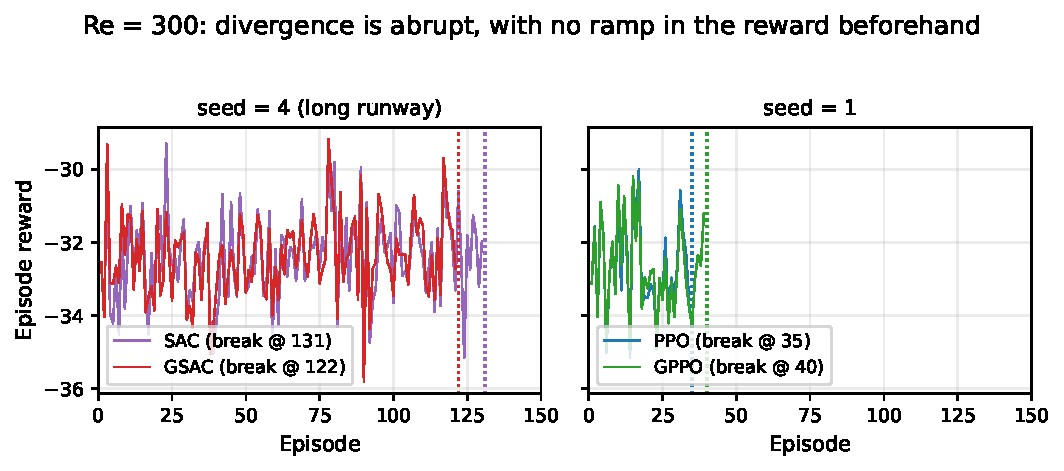
\includegraphics[width=\linewidth]{fig_re300_curves.pdf}
\caption{Example $\Re=300$ training curves. Left: the two long-runway
$\text{seed}=4$ off-policy runs (SAC breaks at episode 131, GSAC at 122).
Right: the $\text{seed}=1$ on-policy runs (PPO at 35, GPPO at 40). In every
case the reward is stationary until a single episode at which it collapses;
the dotted line marks the first-NaN episode.}
\label{fig:re300curves}
\end{figure}

The episode at which this collapse occurs is summarized across all seeds and
algorithms in \cref{fig:breakpoint}.

\begin{figure}[t]
\centering
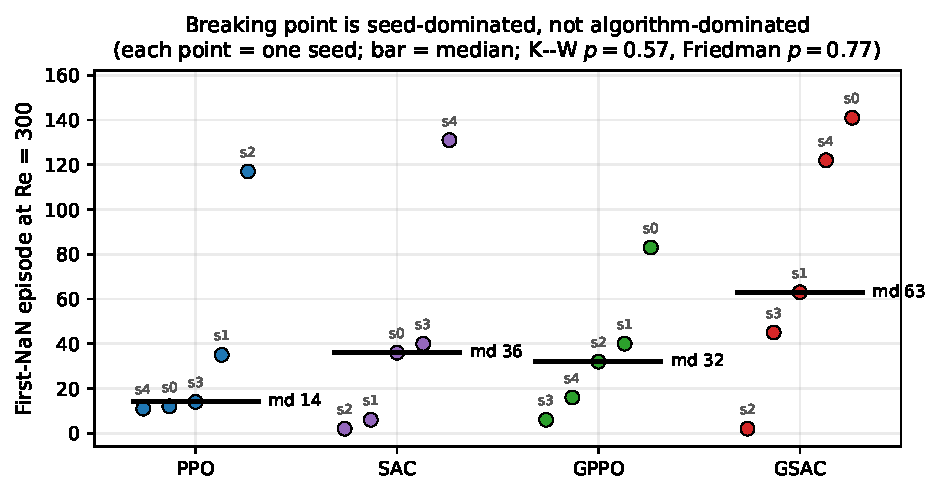
\includegraphics[width=0.86\linewidth]{fig_re300_breakpoint.pdf}
\caption{First-NaN episode at $\Re=300$: each point is one seed, the
horizontal bar is the per-algorithm median. Every algorithm's range spans
more than an order of magnitude, the medians overlap heavily, and no
omnibus test detects an algorithm effect (Kruskal--Wallis $p=0.57$, Friedman
$p=0.77$). GSAC has the highest median but is tied-last at $\text{seed}=2$.}
\label{fig:breakpoint}
\end{figure}

\Cref{tab:breakpoint} lists the exact per-seed episode counts underlying
this figure, together with the per-seed most-robust algorithm.

\begin{table*}[t]
\centering
\caption{First-NaN episode at $\Re=300$ across the five seeds, with
per-algorithm median and mean. ``Most robust'' $=$ latest break in that seed.}
\label{tab:breakpoint}
\small
\resizebox{\textwidth}{!}{%
\begin{tabular}{|l|c|c|c|c|c|c|c|}
\hline
Algorithm & seed$=0$ & seed$=1$ & seed$=2$ & seed$=3$ & seed$=4$ & median & mean \\
\hline
PPO  & 12  & 35 & 117 & 14 & 11  & 14 & 37.8 \\
\hline
SAC  & 36  & 6  & 2   & 40 & 131 & 36 & 43.0 \\
\hline
GPPO & 83  & 40 & 32  & 6  & 16  & 32 & 35.4 \\
\hline
GSAC & 141 & 63 & 2 & 45 & 122 & 63 & 74.6 \\
\hline
most robust & GSAC & GSAC & PPO & GSAC & SAC & --- & --- \\
\hline
\end{tabular}%
}

\end{table*}

At $n=2$ (the conference version) two claims survived: analytic-gradient
injection delays the break (GPPO $>$ PPO, GSAC $>$ SAC) in direction, and
GSAC is the most robust of the four. At $n=5$ neither is a
statistically separable ordering.

Analytic-gradient injection does not delay the on-policy break: GPPO $>$
PPO holds at seeds 0, 1, 4 (83 vs 12; 40 vs 35; 16 vs 11) but
reverses hard at $\text{seed}=2$ (32 vs 117) and $\text{seed}=3$ (6 vs 14,
GPPO breaking first of all four). The paired per-seed difference GPPO$-$PPO
is $\{+71,+5,-85,-8,+5\}$, mean $\mathbf{-2.4}$ episodes, sign-flip
permutation $p=\mathbf{0.81}$.

GSAC leads by median but not significantly: its breaking point (median 63,
mean 74.6) is the highest of the four; it
is the most robust algorithm at seeds 0, 1, 3, second at $\text{seed}=4$, and
tied-last at $\text{seed}=2$ (the early-init failure mode of
\cref{sec:earlyinit} --- the flow diverges before learning begins and bare
SAC fails identically at the same episode). But the spread is enormous:
GSAC$-$SAC per seed is $\{+105,+57,0,+5,-9\}$, $p=0.38$; GSAC$-$GPPO is
$\{+58,+23,-30,+39,+106\}$, $p=0.19$; GSAC$-$PPO $p=0.38$.

What does hold across all five seeds are three seed-stable statements. Every algorithm eventually diverges at
$\Re=300$: analytic-gradient injection never prevents the break, it at most
postpones it. The break is never preceded by a visible precursor in the
reward or gradient signal (\cref{sec:precursor}). And the breaking point is
dominated by the seed --- within-algorithm variance across seeds (s.d.\
30--57 episodes) swamps the between-algorithm differences in mean (spread of
means 35--75). The ``clean multiplicative'' structure reported at $n=1$ and the ``GSAC most
robust'' claim that survived $n=2$ are both artifacts of small $n$. GSAC
carries a non-significant robustness lean --- highest median, most robust in
3/5 --- reported as a candidate effect, not a claim.

\subsection{Significance test ($n=5$)}
\label{sec:sig}

\Cref{tab:sig} gives the full pairwise comparison.

\begin{table*}[t]
\centering
\caption{Pairwise breaking-point comparison at $\Re=300$, $n=5$. Exact
sign-flip permutation $p$ (two-sided); bootstrap \SI{95}{\percent} CI for the
median difference.}
\label{tab:sig}
\small
\resizebox{\textwidth}{!}{%
\begin{tabular}{|l|c|c|c|c|c|}
\hline
Comparison & per-seed diff (s0--s4) & mean & median & \SI{95}{\percent} CI (median) & $p$ \\
\hline
GPPO $-$ PPO  & $+71,+5,-85,-8,+5$      & $-2.4$  & $+5$  & $[-85,+71]$   & 0.81 \\
\hline
GSAC $-$ SAC  & $+105,+57,0,+5,-9$      & $+31.6$ & $+5$  & $[-9,+105]$   & 0.38 \\
\hline
GSAC $-$ GPPO & $+58,+23,-30,+39,+106$  & $+39.2$ & $+39$ & $[-30,+106]$  & 0.19 \\
\hline
GSAC $-$ PPO  & $+129,+28,-115,+31,+111$& $+36.8$ & $+31$ & $[-115,+129]$ & 0.38 \\
\hline
SAC $-$ PPO   & $+24,-29,-115,+26,+120$ & $+5.2$  & $+24$ & $[-115,+120]$ & 0.88 \\
\hline
GPPO $-$ SAC  & $+47,+34,+30,-34,-115$  & $-7.6$  & $+30$ & $[-115,+47]$  & 0.88 \\
\hline
\end{tabular}%
}

\end{table*}

Omnibus: Kruskal--Wallis $H=2.00$, $p=0.57$; Friedman $\chi^2=1.80$,
$p=0.77$. No pairwise or omnibus comparison reaches $p<0.05$. Per
the pre-registered decision rule (\cref{sec:intro}), the finding stands as
no statistically separable ordering of chaotic-regime training
stability by algorithm. GSAC's non-significant lean (highest median and
mean, most robust in 3/5 seeds, all pairwise $p\in[0.19,0.38]$) is reported
as a candidate effect for a future larger-$n$ study.

\subsection{Analytic-gradient norm}
\label{sec:gradnorm}

\Cref{fig:gradnorm} plots the analytic-gradient norm $\lVert\gan\rVert$ over
training, up to the break, for GPPO and GSAC in both regimes. Contrary to the
pre-registered hypothesis, $\lVert\gan\rVert$ does \emph{not} blow up before
the break at $\Re=300$: it fluctuates in the same $\sim$20--70 band as at
$\Re=45$ and shows no upward trend approaching the divergence episode. The
instability that ends training is therefore not visible in the gradient
magnitude --- a point developed mechanistically in \cref{sec:mechanism}.

\begin{figure}[t]
\centering
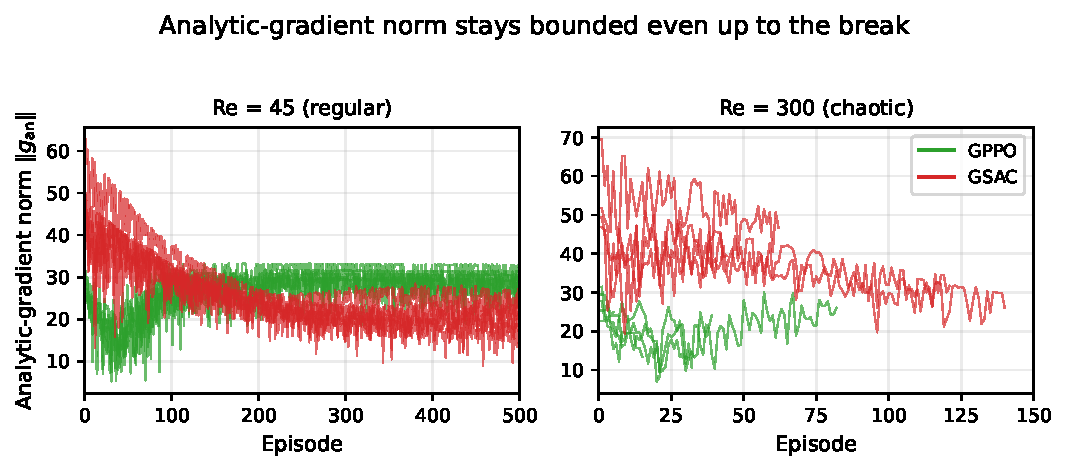
\includegraphics[width=\linewidth]{fig_gradnorm.pdf}
\caption{Analytic-gradient norm $\lVert\gan\rVert$ per episode (all five
seeds overlaid), truncated at each run's first-NaN episode. Left: $\Re=45$.
Right: $\Re=300$. The norm stays bounded and trend-free right up to the
break; the chaotic-regime divergence is not preceded by a gradient
explosion.}
\label{fig:gradnorm}
\end{figure}

\section{Mechanism of the break}
\label{sec:mechanism}

\Cref{sec:precursor,sec:buffer} are direct inspections of raw training
curves; \cref{sec:earlyinit} uses the per-episode action-amplitude log
(\cref{sec:gsac,sec:setup}). \Cref{fig:mechanism} summarizes the two
surviving mechanistic results.

\subsection{The break is sudden and precursor-free}
\label{sec:precursor}

For all four algorithms, in every seed with a mid-training break (seeds 0, 1,
3, 4), the mean and standard deviation of the reward are stable over the
40-episode window immediately before the break --- no ramp, no gradual
degradation (\cref{tab:prebreak}). The longest-runway confirmations come from
$\text{seed}=4$, where \texttt{sac\_high} (break at 131) and
\texttt{gsac\_high} (break at 122) each have a full 40-episode pre-break
window flat to within noise: $-32.29\!\to\!-32.32$ (s.d.\ 1.09) and
$-32.29\!\to\!-32.08$ (s.d.\ 1.18) respectively (\cref{fig:mechanism}a).

\begin{table*}[t]
\centering
\caption{Pre-break reward statistics (40-episode window where the runway
allows, else the full pre-break run; seed $=0\,/\,1\,/\,4$).}
\label{tab:prebreak}
\small
\resizebox{\textwidth}{!}{%
\begin{tabular}{|l|c|c|c|}
\hline
Algorithm & First-half mean & Second-half mean & Std.\ dev. \\
\hline
PPO  & $-32.75\,/\,{-32.28}\,/\,{-32.36}$ & $-32.77\,/\,{-33.05}\,/\,{-32.39}$ & $1.35\,/\,1.32\,/\,0.91$ \\
\hline
SAC  & $-33.31\,/\,{-32.76}\,/\,{-32.29}$ & $-32.50\,/\,{-32.79}\,/\,{-32.32}$ & $1.30\,/\,1.39\,/\,1.09$ \\
\hline
GPPO & $-32.61\,/\,{-32.38}\,/\,{-32.60}$ & $-32.98\,/\,{-33.01}\,/\,{-33.05}$ & $1.10\,/\,1.24\,/\,1.34$ \\
\hline
GSAC & $-32.49\,/\,{-32.19}\,/\,{-32.29}$ & $-32.46\,/\,{-32.08}\,/\,{-32.08}$ & $1.32\,/\,1.16\,/\,1.18$ \\
\hline
\end{tabular}%
}

\end{table*}

GPPO/GSAC analytic-gradient norms over the 15 episodes before the break are
similarly flat (\cref{fig:gradnorm}). The break is therefore not the policy
\emph{gradually} driving the solver past its limit, but a sudden, stochastic
event --- a single episode's randomly sampled action sequence, combined with
the current policy, pushing the flow past the solver's $\Re\approx 350$--$380$
numerical-stability limit (\cref{sec:env}) --- consistent with the
butterfly-effect trigger expected from Metz et al.~\cite{metz2021} and the
Re-shrunk predictability horizon of Boffetta and Musacchio~\cite{boffetta2017}.

\subsection{On-policy vs.\ off-policy after the trigger: buffer dilution}
\label{sec:buffer}

In on-policy PPO/GPPO the trigger episode's rollout is used in that same
episode's update, so trigger and permanent collapse always coincide --- no
escape, in any of the 10 on-policy runs (\cref{tab:trigger}). Off-policy
training \emph{could} in principle dilute the poisoned transitions in its
replay buffer. Whether it does depends on how full the buffer is at the
trigger. Let a run trigger at episode $e$, so the buffer holds $\approx 15e$
transitions of which $\approx 15$ are poisoned; the probability that
\emph{none} of the $10\times 64 = 640$ sampled transitions across the 10
post-trigger updates is poisoned is
\begin{equation}
  P_{\text{survive}}(e)\;\approx\;\left(1-\frac{15}{15\,e}\right)^{640}
  \;=\;\left(1-\frac{1}{e}\right)^{640}.
  \label{eq:survive}
\end{equation}
\Cref{eq:survive} is negligible unless $e\gtrsim 120$ (\cref{fig:mechanism}b):
a run triggering at episode 36 has $P_{\text{survive}}\approx 0$, whereas one
triggering at episode 141 has $P_{\text{survive}}\approx 1\%$. Only GSAC
triggers late enough (seeds 0 and 4, episodes 141 and 122) for this to be
non-negligible.

\begin{table}[t]
\centering
\caption{Trigger episode vs.\ recovery. ``Recovered'' $=$ intermediate
episodes with a valid (non-NaN) reward between trigger and permanent
collapse. Across all 20 $\Re=300$ runs exactly one shows a recovery window:
$\text{seed}=0$ GSAC (2 episodes).}
\label{tab:trigger}
\small
\begin{tabular}{|l|c|c|}
\hline
Algorithm & Trigger (s0\,/\,s1\,/\,s2\,/\,s3\,/\,s4) & Recovered \\
\hline
PPO  & $12\,/\,35\,/\,117\,/\,14\,/\,11$   & $0\,/\,0\,/\,0\,/\,0\,/\,0$ \\
\hline
SAC  & $36\,/\,6\,/\,2\,/\,40\,/\,131$     & $0\,/\,0\,/\,0\,/\,0\,/\,0$ \\
\hline
GPPO & $83\,/\,40\,/\,32\,/\,6\,/\,16$     & $0\,/\,0\,/\,0\,/\,0\,/\,0$ \\
\hline
GSAC & $141\,/\,63\,/\,2\,/\,45\,/\,122$   & $\mathbf{2}\,/\,0\,/\,0\,/\,0\,/\,0$ \\
\hline
\end{tabular}
\end{table}

\Cref{fig:mechanism}b plots \cref{eq:survive} against the actual trigger
episodes of the ten off-policy runs in \cref{tab:trigger}, with the single
observed recovery window circled.

\begin{figure}[t]
\centering
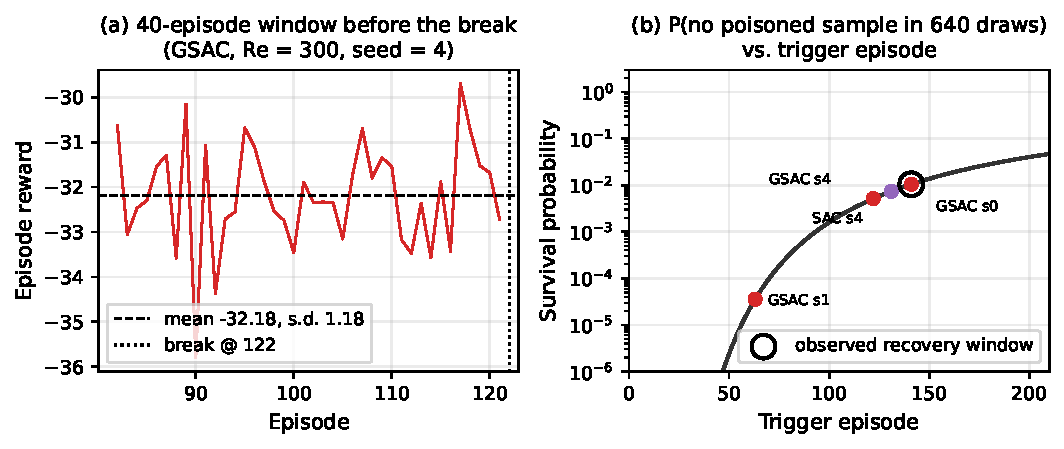
\includegraphics[width=\linewidth]{fig_mechanism.pdf}
\caption{Two surviving mechanistic results. (a) The 40-episode reward window
before the break (GSAC, $\Re=300$, $\text{seed}=4$): flat to within noise,
then an abrupt divergence. (b) The buffer-dilution survival probability of
\cref{eq:survive} vs.\ trigger episode; markers are the actual off-policy
runs, and the single observed recovery window (circled, $\text{seed}=0$
GSAC, trigger 141) is the one case where $P_{\text{survive}}$ is $\sim$1\%.}
\label{fig:mechanism}
\end{figure}

\Cref{eq:survive} gives a non-zero survival
probability only for a GSAC run that triggers past $\sim$episode 120. Two of
the five GSAC runs meet this ($\text{seed}=0$ at 141, $\text{seed}=4$ at 122);
the model predicts a recovery window is \emph{possible but rare} ($\sim$1\%)
for these and effectively impossible for the other 18 runs. Observed: one
window, in $\text{seed}=0$ GSAC. This is consistent with the model, but with
one positive across 20 runs the mechanism is suggestive, not
confirmed; a controlled buffer-size sweep at a fixed trigger is needed to
establish the $\sim$1\% rate.

\subsection{Divergence before learning: the early-init failure mode}
\label{sec:earlyinit}

The $\text{seed}=2$ sweep exposes a second, qualitatively different failure
mode. In $\text{seed}=2$ at $\Re=300$, both SAC and GSAC break at
episode 2 with an \emph{identical} episode-1 trajectory: same reward
($-33.68$), same action RMS ($0.308$), same action abs-max ($0.489$). This
identity is expected --- SAC and GSAC share the seed's initialization and
diverge only after episode 1, when GSAC applies its extra analytic step ---
yet both reach NaN on episode 2.

The logs rule out the \cref{sec:buffer} mechanism and an action-explosion
mechanism alike. GSAC's episode-1 analytic-gradient norm is 54,
squarely in the normal range ($\text{seed}=0$: 49, $\text{seed}=1$: 69 over
their first ten episodes), so the analytic step was not anomalous; and the
episode-2 rollout's action RMS is 0.307 with abs-max 0.485,
indistinguishable from episode 1, so the policy is not driving the flow with
large control.
What remains is that $\text{seed}=2$'s randomly initialized policy, composed
with the $\Re=300$ base flow, integrates to numerical divergence within two
episodes --- before any actor-learning algorithm has a foothold. Bare SAC
diverges identically, so this is a property of where the random
initialization lands relative to the solver's stability boundary
(\cref{sec:env}), not of analytic-gradient injection. GSAC's long runways in
seeds 0, 1, 4 (141, 63, 122 episodes) require several non-diverged episodes
for the analytic gradient to accumulate a stabilizing effect; $\text{seed}=2$
provides no such runway.

This mode is rare: 1 of 5 seeds. Seeds 3 and 4 both break
mid-training, so the episode-2 collapse is not the typical $\Re=300$
behaviour --- it is a low-probability tail of the same sudden,
precursor-free, stochastic trigger of \cref{sec:precursor}, occurring at
episode 2 instead of 45--141. It still reframes GSAC as highest
ceiling, no reliable floor, and shows the trigger-episode distribution
reaches all the way down to episode 2.

\Cref{sec:buffer} is a plausibility calculation
for the post-trigger lock-in; \cref{sec:earlyinit} shows \emph{when} the
trigger can occur. Neither explains \emph{why} a given (seed, init) triggers
at a given episode. The action-amplitude log now in place is the instrument
for this; a dedicated short-horizon re-run of seeds 0--1 logging the per-step
action norm is the next diagnostic (\cref{sec:conclusion}).

\section{Discussion}
\label{sec:discussion}

This work extends the HydroGym paper's GPPO-vs-PPO result on Kolmogorov
flow~\cite{hydrogym2026} in two directions, and the second produces a
seed-dominance result that is itself the main finding.

At the regular operating point ($\Re=45$) the paper's core claim holds: GPPO reaches
PPO's best reward in substantially fewer episodes in 4 of 5 seeds
($\approx$\SIrange{63}{84}{\percent}, $\text{seed}=0$'s \SI{63}{\percent}
closest to the reported \SI{65}{\percent}), the direction is seed-stable
across all five, and the off-policy family reaches better final reward than
the on-policy family in every seed. GSAC never beats SAC here --- the
analytic gradient does not help the off-policy method when the flow is not
chaotic. This is consistent with the SAPO~\cite{sapo2025} reading that the
analytic gradient earns its keep by \emph{stabilizing} a hard landscape
rather than by accelerating an easy one; at $\Re=45$ SAC's replay buffer
already solves the task.

At the chaotic operating point ($\Re=300$), by contrast, no separable
ordering survives: the conference version, at $n=2$, reported that GSAC is
the most robust of the four and that analytic-gradient injection delays the
break in direction.
Over five seeds the second claim does not hold at all (GPPO$-$PPO mean
$-2.4$ episodes, sign-flip $p=0.81$) and the first survives only as a
non-significant lean (every pairwise permutation $p\ge 0.19$;
Kruskal--Wallis $p=0.57$, Friedman $p=0.77$). Each algorithm's first-NaN
episode spans more than an order of magnitude; PPO, first to break at
$\text{seed}=0$, is the most robust of the four at $\text{seed}=2$; at
$\text{seed}=2$ both off-policy methods collapse at episode 2. The ``clean
multiplicative'' $n=1$ story and the ``GSAC most robust'' $n=2$ story are
both small-$n$ artifacts. The finding that replaces them: in the
chaotic regime the breaking point is dominated by the random path of
training, not by the algorithm --- within-algorithm cross-seed s.d.\
(30--57 episodes) swamps the spread of between-algorithm means (35--75).
Analytic-gradient injection, off-policy structure, and their combination
fail to impose a statistically separable ordering on when a differentiable
chaotic-flow simulation diverges under RL training. This is a concrete,
quantified instance of the chaos-induced gradient instability of Metz et
al.~\cite{metz2021} and the Re-shrunk predictability horizon of
Boffetta--Musacchio~\cite{boffetta2017}: at this problem scale the
instability is not merely large, it is \emph{irreducibly stochastic}. It
also matches what RPO~\cite{rpo2025} targets --- the training instability of
BPTT-through-a-surrogate --- and suggests that the RPO/GI-PPO line of
adaptive weighting, rather than a fixed mix, is the right tool for this
regime.

Two mechanistic results do survive, both algorithm-design-independent. The
first is buffer dilution
(\cref{sec:buffer}): a post-trigger survival window has non-zero probability
only when the poisoned fraction of the replay buffer at the trigger is
$\sim$1\% or below --- that is, only for GSAC runs that trigger past
$\sim$episode 120 --- and exactly one of the 20 $\Re=300$ runs shows such a
window, in precisely that case, so the mechanism is suggestive rather than
confirmed. The second is the early-init failure mode (\cref{sec:earlyinit}):
when the randomly initialized policy composed with the $\Re=300$ base flow
already sits near the solver's stability boundary, divergence occurs within
about two episodes, before any actor-learning algorithm has a foothold; bare
SAC and GSAC fail identically here, with normal control amplitude and a
normal analytic-gradient norm at the point of divergence. Together these
explain why GSAC has the highest ceiling of the four (141, 63, and 122
episodes when it is given a runway) but no reliable floor (episode 2 at
$\text{seed}=2$).

For a practitioner adding an analytic through-simulator gradient to an RL
controller for a near-turbulent flow: (i) expect no reliable improvement in
training stability from the gradient alone, and budget for divergence at an
unpredictable episode; (ii) an off-policy buffer buys a recovery chance only
if the divergence happens late, when the buffer is large --- it is not a
general safety net; and (iii) the useful engineering artifacts are the
diagnostics (first-NaN-episode distribution, pre-break flatness check,
buffer-dilution estimate), not a ranking of algorithms. None of this refutes
the HydroGym paper's core claim that GPPO helps at its tested operating
point; it shows the benefit does not carry a seed-robust ordering once the
regime is chaotic.

Several caveats bound these conclusions. The study uses five seeds: this is
enough to falsify the $n=2$ orderings and to support the negative claim, but
GSAC's non-significant median lean ($p\approx0.19$--$0.38$) would need a
substantially larger seed budget to confirm or reject --- though, because the
finding is one of seed-dominance, additional seeds are expected to strengthen
it rather than overturn it. The chaotic regime is $\Re=300$ rather than the
originally intended $\Re=450$, forced by the solver's $\Re\approx350$--$380$
stability limit at this grid and time step; a milder chaotic regime might
admit a more stable ordering, which the planned Reynolds sweep
$\{45,100,200,300\}$ is designed to test. The GPPO/GSAC mixing ratio,
horizon, and remaining hyperparameters are our own choices, since the
HydroGym paper does not publish them, so the \SI{63}{\percent} versus
\SI{65}{\percent} agreement is a strong corroborating signal but not a claim
of identical implementation. The PPO update is deliberately minimal (one
full-batch step per episode), which makes ``PPO'' here weaker than a tuned
implementation; the comparison is therefore relative and budget-matched
across all four algorithms rather than absolute. The episodes (15 RL steps)
and the analytic horizon (6 steps) are both short and may be insufficient to
observe the full course of RL convergence or of chaotic divergence, and the
50/50 analytic/model-free mix is held fixed --- the adaptive $\alpha$-graded
estimator~\cite{suh2022}, AHAC's~\cite{ahac2024} adaptive horizon, and
SAPO's~\cite{sapo2025} entropy-based smoothing are not tested. Finally, the
two mechanistic results rest on thin evidence: the buffer-dilution
calculation of \cref{sec:buffer} is supported by a single recovery window in
20 runs, and the early-init failure of \cref{sec:earlyinit} by a single
seed; both are real but rare, and neither is established as a rate.

\section{Conclusion and future work}
\label{sec:conclusion}

Analytic-gradient injection does not eliminate numerical instability in the
chaotic regime and, across independent training seeds, does not reliably
delay the break either. On-policy injection has no measurable effect on the
breaking point, and while the gradient-enhanced off-policy method GSAC has
the highest median breaking point and is the most robust of the four in most
seeds, no pairwise or omnibus test reaches significance; the ordering
suggested by a small seed budget does not survive a larger one. The
reproducible statement is one of seed-dominance: in the chaotic regime the
episode at which training first diverges is dominated by the random path of
training, not by the algorithm. What survives is mechanistic: the break is
sudden and precursor-free; the replay buffer's size at the trigger sets
whether a brief post-trigger survival window can appear; and in a rare mode
the flow diverges within a couple of episodes regardless of algorithm because
the random initial policy already sits near the solver's stability boundary.
On this evidence GSAC has the highest ceiling of the four but no reliable
floor.

Five directions follow directly. First, extend well beyond five seeds to
test GSAC's non-significant median lean; the seed-dominance of the breaking
point means a decisive test needs many seeds. Second, resolve the
trigger-episode cause with an action-amplitude-logged short-horizon re-run of
seeds 0--1 --- is the trigger a single large sampled action or a resonant
sequence? Third, test whether GSAC's floor can be raised (not its ceiling)
with cheap, principled guards: analytic-gradient norm clipping, a
non-finite-gradient fallback to pure SAC, a few-episode analytic warmup, and
an adaptive mixing weight in the style of the GI-PPO $\alpha$-policy or of
AHAC / SAPO. Fourth, run a Reynolds sweep $\{45,100,200,300\}$ to locate the
Reynolds number at which any algorithm ordering disappears, framed with the
predictability-horizon scaling of Boffetta and Musacchio. Fifth, reconcile
against the official HydroGym GPPO implementation and a stronger PPO baseline
with epochs and minibatching, and extend the comparison to a second
environment.


\section*{Acknowledgment}
The authors thank Sakarya University's National Technology Workshop
Artificial Intelligence Center for the computational resources used in this
study.

\section*{Funding}
This research did not receive any specific grant from funding agencies in the
public, commercial, or not-for-profit sectors.

\section*{Declaration of generative AI and AI-assisted technologies in the writing process}
During the preparation of this work the authors used Claude (Anthropic) in order
to improve the language and readability of the manuscript and to assist with
code and figure generation. After using this tool, the authors reviewed and
edited the content as needed and take full responsibility for the content of
the published article.

\section*{Declaration of competing interest}
The authors declare no competing interests.

\section*{Data and code availability}
The experiment code, pinned environment specification, sweep drivers, and
every per-configuration result dump (episode rewards, analytic-gradient
norms, action-amplitude logs, wall times) are publicly available at
\url{https://github.com/GulogluHaktan/hydrogym-work}. A permanent archive with
a DOI will be added before final publication.

\printcredits

\bibliographystyle{elsarticle-num}
\bibliography{refs}

%% Biographies follow the author order.  Each \bio{} still needs its photo
%% file: save it next to main.tex and change \bio{} to \bio{<filename>},
%% matching the \bio{photo-haktan} pattern used for the last author.  JAI
%% requires a photograph for every author of a full-length article.
\bio{}
Cem \"Ozkurt is a researcher in the Department of Data Science and Analytics,
Faculty of Computer and Information Sciences, Sakarya University. He conceived
and designed the study, led its methodology and administered the project.
\endbio

\bio{}
Muhammed Emin Onay is affiliated with the Department of Computer Engineering,
Faculty of Computer and Information Sciences, Sakarya University. In this study
he contributed to the curation of the per-run experimental data and to the
visualisation of the breaking-point and gradient-norm results.
\endbio

\bio{}
Ey\"up Altu\u{g} Tun\c{c} is affiliated with the Department of Computer
Engineering, Faculty of Computer and Information Sciences, Sakarya University.
In this study he contributed to the software implementation and to the
validation of the training pipeline across the five seeds.
\endbio

\bio{}
Ahmet Kutay K\"u\c{c}\"ukler is affiliated with the Department of Computer
Engineering, Sakarya University of Applied Sciences. In this study he
contributed to the experimental runs and to the validation of the results.
\endbio

\bio{photo-haktan}
Haktan Yusuf G\"ulo\u{g}lu graduated at the top of his class from Profilo
Vocational and Technical Anatolian High School and is currently an
undergraduate student in the Department of Computer Engineering, Sakarya
University of Applied Sciences. His research centers on reinforcement
learning and large language models, with a particular interest in the
stability of learning algorithms under complex, high-dimensional, and
chaotic dynamics. This work is his first contribution to the
differentiable-simulation reinforcement learning literature.
\endbio

\end{document}
